\documentclass[12pt]{article}
\usepackage[utf8]{inputenc}
\usepackage[T1]{fontenc}
\usepackage{textcomp}
\DeclareUnicodeCharacter{20A1}{\textcent}% símbolo del colón (₡), se imprime como ¢ como en el pliego del ICE
\usepackage[spanish,es-nodecimaldot]{babel}
\usepackage{lmodern}
\usepackage[a4paper,margin=2.3cm]{geometry}
\usepackage{setspace}
\usepackage{graphicx}
\usepackage{float}
\usepackage{booktabs}
\usepackage{longtable}
\usepackage{array}
\usepackage{tabularx}
\usepackage{multirow}
\usepackage{siunitx}
\usepackage{amsmath,amssymb}
\usepackage{xcolor}
\usepackage{enumitem}
\setlist{itemsep=2pt,topsep=3pt,parsep=0pt}
\usepackage{fancyhdr}
\usepackage{tikz}
\usetikzlibrary{arrows.meta,positioning,shapes.geometric,calc,babel}
\usepackage{caption}
\usepackage{subcaption}
\usepackage{pdflscape}
\usepackage{titlesec}
\usepackage{lastpage}
\usepackage{microtype}
\usepackage{fancyvrb}
\usepackage{xurl}
\usepackage{hyperref}
\setlength{\emergencystretch}{2em}

\hypersetup{colorlinks=true,linkcolor=black,urlcolor=blue,citecolor=black}
\sisetup{output-decimal-marker={,},group-separator={\,},group-minimum-digits=4,per-mode=symbol}
\setstretch{1.12}
\setlength{\parindent}{0pt}
\setlength{\parskip}{0.55em}
\pagestyle{fancy}
\fancyhf{}
\lhead{EL-4601 Normalización Técnica para Electrónica}
\rhead{Proyecto No. 3}
\cfoot{\thepage\ de \pageref{LastPage}}
\setlength{\headheight}{15pt}
\fancypagestyle{lscape}{\fancyhf{}\lhead{EL-4601 Normalización Técnica para Electrónica}\rhead{Proyecto No. 3}\cfoot{\thepage\ de \pageref{LastPage}}}
\titleformat{\section}{\Large\bfseries}{\thesection.}{0.5em}{}
\titleformat{\subsection}{\large\bfseries}{\thesubsection.}{0.5em}{}
\titleformat{\subsubsection}{\normalsize\bfseries}{\thesubsubsection.}{0.5em}{}
\captionsetup{font=small,labelfont=bf}
\newcolumntype{L}[1]{>{\raggedright\arraybackslash}p{#1}}
\newcolumntype{Y}{>{\raggedright\arraybackslash}X}
\newcolumntype{R}[1]{>{\raggedleft\arraybackslash}p{#1}}

% Marca de los supuestos de diseño (Cuadro~\ref{tab:supuestos}).
\newcommand{\supuesto}{\textsuperscript{\textcolor{orange!80!black}{\textbf{(S)}}}}
% Lámina A3 en página horizontal
\newcommand{\lamina}[3]{%
\begin{landscape}\thispagestyle{lscape}
\begin{figure}[p]\centering
\includegraphics[width=\linewidth,height=0.86\textheight,keepaspectratio]{#1}
\caption{#2}\label{#3}
\end{figure}
\end{landscape}}

\begin{document}

% =====================================================================
\begin{titlepage}
\centering
\vspace*{1.2cm}
{\Large Instituto Tecnológico de Costa Rica\\[0.3cm]}
{\large Unidad de Ingeniería Electrónica -- Centro Académico de Alajuela\\[1.0cm]}
{\large EL-4601 Normalización Técnica para Electrónica\\[0.5cm]}
{\LARGE\bfseries Proyecto No. 3\\[0.35cm]}
{\LARGE\bfseries Cargadores para vehículos eléctricos\\[0.2cm]}
{\Large Investigación normativa y diseño en Costa Rica\\[0.4cm]}
{\large Estación de carga de uso público en el parqueo norte del campus UTN Villa Bonita (CAA-TEC):\\ cuatro puntos de carga en CA y un cargador rápido de CC de \SI{60}{\kilo\watt}\\[1.5cm]}

\begin{tabular}{rl}
\textbf{Integrantes:} & Walter Alfaro Ulate -- carné 2023073145\\
& Sebastián Meneses Castillo -- carné 2024139307\\
& Thomas Reed Víquez -- carné 2023210321\\
\textbf{Profesor:} & Luis Roberto Pereira Arroyo\\
\textbf{Fecha:} & 4 de noviembre de 2026\\
\end{tabular}

\vfill
{\small Alajuela, Costa Rica -- II Semestre 2026}
\end{titlepage}

\tableofcontents
\clearpage
\listoffigures
\listoftables
\clearpage

% =====================================================================
\section{Resumen ejecutivo}

Este documento investiga las tecnologías y modalidades de carga de vehículos eléctricos (VE), el marco legal y técnico que rige su instalación en Costa Rica, y los equipos y vehículos disponibles. Con esa base, diseña una \textbf{estación de carga de uso público} en el parqueo norte del campus de la Universidad Técnica Nacional (UTN) en Villa Bonita de Alajuela, donde funciona el Centro Académico de Alajuela del TEC (CAA-TEC). Es el mismo campus del Proyecto~2, por lo que se reutilizan los datos verificados del sistema eléctrico: el transformador de pedestal del ICE N.\textsuperscript{o} 119688 (\SI{750}{\kilo\volt\ampere}, 34,5~kV/480Y/277~V), la lámina as-built E01 y el registro fotográfico del 5 de octubre de 2026. La estación se dibujó sobre una imagen satelital descargada para este trabajo (Esri World Imagery, \SI{0.29}{\meter} por píxel).

\textbf{Solución propuesta.}
\begin{itemize}
\item Seis espacios de carga en el extremo este de la fila sur del parqueo, con un espacio accesible (Ley 7600).
\item \textbf{AC-1 y AC-2:} dos cargadores de CA Autel MaxiCharger AC Elite con conector SAE J1772 (Tipo~1), alimentados a 208~V y ajustados a \SI{40}{\ampere} (\SI{8.3}{\kilo\watt}). Tienen listado UL 2594 y UL 2231.
\item \textbf{AC-3 y AC-4:} dos cargadores de CA con conector GB/T (\SI{32}{\ampere}, \SI{6.7}{\kilo\watt}) para la flota china que se vende oficialmente en el país, como el BYD Dolphin, cuya ficha costarricense declara puerto GB/T. Como no tienen listado UL, llevan aguas arriba un diferencial tipo~B de 30~mA.
\item \textbf{DC-1:} un cargador rápido Autel MaxiCharger DC Fast de \SI{60}{\kilo\watt} a 480~V con conectores CCS1 y CHAdeMO (UL 2202). Reparte la potencia (30 + \SI{30}{\kilo\watt}) cuando atiende dos vehículos a la vez.
\item Servicio nuevo e independiente del CAA, desde el nicho del transformador 119688: medición indirecta del ICE, interruptor IP-VE de \SI{200}{\ampere}, alimentador de 3\#3/0 Cu de unos \SI{120}{\meter} \supuesto{} y celda eléctrica en la estación con el tablero TD-VE (480Y/277~V), un transformador seco T-VE de \SI{45}{\kilo\volt\ampere} (480$\Delta$--208Y/120~V) y el tablero TD-AC.
\item Sistema de gestión de energía (EMS, NEC 625.42) que limita la estación a \SI{60}{\kilo\watt} por medio de OCPP.
\end{itemize}

\textbf{Resultados principales.}
\begin{itemize}
\item Demanda máxima de \SI{94.5}{\kilo\watt} sin gestión y de \SI{60}{\kilo\watt} con el EMS. El alimentador de \#3/0 (\SI{200}{\ampere}) cubre el 125\,\% de la carga continua (\SI{182.8}{\ampere}). La caída de tensión es de 1,54\,\% en el alimentador y de 2,79\,\% en el peor ramal, ambas dentro del criterio de 3\,\% y 5\,\%.
\item Tiempos de carga del 20 al 80\,\% (cálculo con la curva de aceptación de cada vehículo, sin suponer potencia constante): BYD Dolphin en CA GB/T, 4~h~32~min; Hyundai Ioniq~5, 6~h~12~min en CA y 48~min en DC-1; Ford F-150 Lightning ER, 10~h~30~min en CA y 1~h~21~min en DC-1; Nissan Leaf, 39~min en CHAdeMO.
\item Corriente de falla de \SI{15.7}{\kilo\ampere} en los bornes del transformador del ICE, \SI{5.8}{\kilo\ampere} en TD-VE y \SI{2.8}{\kilo\ampere} en TD-AC, todas menores que la capacidad interruptiva de cada equipo.
\item Presupuesto referencial de \textbf{USD~102\,500} (unos ₡51,8 millones) antes de impuestos, con 10\,\% de imprevistos. Con la tarifa T-CO del ICE y sin EMS, el cargo por demanda es el 54\,\% de la factura de la estación. Con el EMS y la tarifa T-CS de las instituciones públicas de educación, el costo de operación baja a unos ₡98/kWh.
\end{itemize}

\textbf{Compatibilidad: el hallazgo que más influyó en el diseño.} En Costa Rica conviven vehículos con J1772/CCS1 (mercado estadounidense), CHAdeMO (Nissan Leaf usados) y GB/T (vehículos chinos). La red del ICE ofrece CCS1, CHAdeMO y GB/T en CC, y sus estaciones nuevas dan prioridad a CCS1 y GB/T. Ningún cargador de CC con listado UL a 480~V que se revisó ofrece GB/T: el Zerova DS lo incluye solo en su versión IEC de 400~V. Por eso los vehículos GB/T se atienden con cargadores de CA propios, y el diseño no confía en adaptadores que el fabricante no haya aprobado.

\textbf{Viabilidad.} La estación es \textbf{técnicamente viable} con la infraestructura del campus, sujeta al estudio de capacidad del ICE sobre el transformador 119688. En lo económico, \textbf{no se paga como negocio} con los precios de referencia de la red del ICE (₡99,70/kWh en CA y ₡141/min en CC): el mejor caso (T-CS con EMS) recupera la inversión en unos 12 años, y con la mitad del uso supuesto no se recupera. Se recomienda como \textbf{servicio institucional} de movilidad sostenible y ejecutarla con el EMS. El precio medio de equilibrio a 10 años, con una tasa del 8\,\%, es de unos ₡145/kWh. La Ley~10937 (2026) ya permite vender el servicio, pero ARESEP todavía no ha fijado la tarifa de la energía para operadores privados.

\textbf{Supuestos y limitaciones.} No se pudieron obtener la capacidad remanente del transformador del ICE, la posición exacta del nicho en sitio, el texto de las normas INTE N121 y N120 (son de pago) ni cotizaciones locales de los equipos. Estos datos se reemplazaron por supuestos declarados (Cuadro~\ref{tab:supuestos}), marcados en el texto con \supuesto{}.

% =====================================================================
\section{Objetivos}
\subsection{Objetivo general}
Diseñar una estación de carga de vehículos eléctricos de uso público para el parqueo norte del campus UTN Villa Bonita, fundamentada en la normativa costarricense vigente, en los datos reales del sitio y en equipos comerciales cuya compatibilidad con los vehículos del país esté verificada.

\subsection{Objetivos específicos}
\begin{itemize}[leftmargin=1.2cm]
\item Explicar y comparar las tecnologías y modalidades de carga, desde la carga residencial a 120~V hasta la carga rápida en CC, la transferencia bidireccional (V2L, V2V, V2H, V2G) y las alternativas emergentes.
\item Identificar las leyes, reglamentos, normas técnicas y requisitos de la distribuidora, del CFIA, de la municipalidad, de Bomberos y de accesibilidad que aplican al caso, verificando la edición, la vigencia y el carácter obligatorio de cada documento.
\item Comparar al menos cuatro cargadores y cinco vehículos de distintos fabricantes, y verificar la compatibilidad por conector, versión y mercado.
\item Diseñar la estación (planta, unifilar, detalles), dimensionar los conductores, las canalizaciones y las protecciones, y calcular la energía, la potencia efectiva y el tiempo de carga.
\item Elaborar el cuadro de cargas, el cuadro de equipos, la lista de materiales, el presupuesto y el costo de operación, y analizar la viabilidad técnica, económica y regulatoria.
\end{itemize}

% =====================================================================
\section{Tecnologías y modalidades de carga}
\label{sec:tecnologias}

\subsection{EVSE, cargador a bordo y cargador externo de CC}
\begin{itemize}
\item \textbf{Equipo de suministro para VE (EVSE).} Es el equipo fijo o portátil que conecta el vehículo a la red: conductores, conector, relés, protección de personas y comunicación. \emph{En CA el EVSE no convierte energía}: solo informa al vehículo, por la señal piloto (\emph{control pilot}, SAE J1772 / IEC 61851-1), cuánta corriente puede tomar, y cierra el circuito cuando hay condiciones seguras \cite{iec61851,sae1772}. En el NEC el término incluye conectores, cables y accesorios (art.~625) \cite{nfpa70}.
\item \textbf{Cargador a bordo (OBC).} Es el rectificador que va dentro del vehículo y convierte la CA del EVSE en la CC de la batería. Su potencia (típicamente de 6,6 a \SI{19.2}{\kilo\watt}) limita la carga en CA, aunque el EVSE pueda entregar más. Por ejemplo, el BYD Dolphin vendido en Costa Rica tiene un OBC de \SI{6.6}{\kilo\watt} \cite{bydDolphin}.
\item \textbf{Cargador externo de CC.} El rectificador está fuera del vehículo, en el equipo de la estación, y entrega CC directamente a la batería sin pasar por el OBC. La potencia la negocia el sistema de gestión de la batería (BMS) del vehículo por comunicación digital: PLC según DIN 70121/ISO 15118 en CCS, CAN en CHAdeMO y GB/T 27930 en GB/T \cite{autelDC,zerova}.
\end{itemize}

\subsection{CA y CC, niveles y modos: sistema de clasificación usado}
En CA la conversión la hace el vehículo; en CC, la estación. Hay dos sistemas de clasificación que se usan en paralelo:
\begin{itemize}
\item \textbf{Niveles (SAE J1772, mercado norteamericano y NEC).} Nivel~1: 120~V CA, hasta \SI{16}{\ampere} (unos \SI{1.9}{\kilo\watt}). Nivel~2: 208/240~V CA, hasta \SI{80}{\ampere} (\SI{19.2}{\kilo\watt}). Carga rápida en CC: desde decenas hasta cientos de kW \cite{sae1772}.
\item \textbf{Modos (IEC 61851-1, adoptada como INTE/IEC 61851-1).} Modo~1: conexión directa a un tomacorriente sin control. Modo~2: cable portátil con dispositivo de control y protección en el cable (IC-CPD). Modo~3: EVSE dedicado de CA con señal piloto. Modo~4: cargador externo de CC \cite{iec61851,intecoBlog}.
\end{itemize}
Este documento usa \textbf{los modos IEC} como clasificación principal, porque el reglamento de la Ley 9518 define los centros de recarga por referencia a INTE/IEC 61851-1, -22 y -23 \cite{dec41428}. Para los equipos norteamericanos se indica además el nivel SAE, que es el lenguaje del NEC y de las fichas UL. Con esa convención, AC-1 a AC-4 son \textbf{Modo~3 / Nivel~2}, DC-1 es \textbf{Modo~4} y un cable portátil de 120~V es \textbf{Modo~2 / Nivel~1}.

\subsection{Carga residencial con tomacorriente de 120 V y equipo portátil}
\begin{itemize}
\item \textbf{Circuito:} tomacorriente NEMA 5-15 o 5-20 en un circuito dedicado de 15 o \SI{20}{\ampere}. Como la carga es continua, la corriente queda limitada al 80\,\% del circuito: 12 o \SI{16}{\ampere} (NEC 625.41 y 210.19). El tomacorriente requiere protección GFCI (625.54) \cite{nfpa70}.
\item \textbf{Potencia:} $120 \times 12 = \SI{1.44}{\kilo\watt}$ en la red, y unos \SI{1.2}{\kilo\watt} en la batería con una eficiencia del 85\,\% \supuesto{}.
\item \textbf{Tiempo de carga:} un Nissan Leaf de \SI{39}{\kilo\watt\hour} útiles necesita unas 19~h para pasar del 20 al 80\,\% ($23{,}4/1{,}22$), y un Hyundai Ioniq~5 (\SI{77.4}{\kilo\watt\hour}), unas 38~h. Solo sirve para recorridos diarios cortos (unos 40--60~km por noche).
\item \textbf{Limitaciones:} calentamiento de tomacorrientes viejos, prohibición de extensiones y pérdidas proporcionalmente mayores. En Costa Rica las viviendas reciben servicio monofásico trifilar de 120/240~V, así que suele ser posible migrar a 240~V.
\end{itemize}

\subsection{Carga residencial con equipo de pared o pedestal (wallbox)}
Es un EVSE Modo~3 conectado a 240~V entre fases (vivienda) o a 208~V entre fases (edificios con servicio 208Y/120~V), en un circuito dedicado al 125\,\% de la corriente del equipo. Con \SI{40}{\ampere} (circuito de \SI{50}{\ampere}) entrega \SI{9.6}{\kilo\watt} a 240~V o \SI{8.3}{\kilo\watt} a 208~V, aunque la potencia real la fija el OBC. A 208~V la potencia baja un 13\,\% con la misma corriente, un efecto que se cuantifica en la sección~\ref{sec:calc_carga}. Antes de instalarlo hay que revisar la capacidad del servicio con el cálculo de cargas (NEC 220) o usar un sistema de gestión de carga (625.42).

\subsection{Condominios, comercios, empresas y estacionamientos}
\begin{itemize}
\item \textbf{Acceso compartido:} los usuarios se identifican con tarjeta RFID o con una aplicación, los equipos se gestionan en red con OCPP 1.6J o 2.0.1, y se fijan reglas de permanencia para liberar los espacios.
\item \textbf{Medición:} hay dos esquemas. En uno, cada usuario tiene su medidor o su circuito asociado a su propio servicio. En el otro, la medición es común y se reparte por sesión con el medidor interno del EVSE (clase~A en DC-1 \cite{autelDC}). La reventa de energía a terceros es un servicio de interés general sujeto a la Ley 10937 y a ARESEP (sección~\ref{sec:ley9518}).
\item \textbf{Gestión de varios puntos:} un EMS reparte la capacidad disponible entre los puntos activos. El NEC 2020 permite dimensionar el alimentador con el límite que fija el EMS (625.42), lo que evita ampliar el servicio. En condominios, la instalación en áreas comunes necesita además la aprobación de los condóminos según su reglamento interno.
\end{itemize}

\subsection{Carga pública rápida y de alta potencia en CC}
\begin{itemize}
\item \textbf{Alimentación:} servicio trifásico, típicamente 480Y/277~V, o 208~V en equipos pequeños. Un equipo de \SI{60}{\kilo\watt} toma unos \SI{91}{\ampere} a 480~V \cite{autelDC}, y uno de \SI{120}{\kilo\watt}, \SI{153}{\ampere} \cite{abbTerra124}. Con frecuencia se necesita un transformador propio y el estudio de capacidad de la distribuidora. El cargo por demanda domina el costo de operación (sección~\ref{sec:economia}).
\item \textbf{Conectores:} CCS1 (Combo~1), CCS2 (Combo~2), CHAdeMO, GB/T y NACS (SAE J3400). La red del ICE ofrece CCS1, CHAdeMO y GB/T \cite{delfinoAresep}.
\item \textbf{Condiciones de operación:} reducción de potencia por temperatura ambiente y de batería, por altitud (sobre los 2000~m) y por estado de carga. Por encima del 50--80\,\% de SOC, la potencia cae.
\item \textbf{Límites del vehículo:} potencia máxima de aceptación, tensión de la batería (400 u 800~V) frente a la corriente máxima del conector (CCS1: \SI{200}{\ampere} en DC-1; CHAdeMO: \SI{125}{\ampere}), y protocolo. Un vehículo de 400~V en un cargador limitado a \SI{200}{\ampere} no pasa de unos \SI{80}{\kilo\watt}.
\end{itemize}

\subsection{Pickups con tomacorrientes de salida de 120/240 V}
Hay que distinguir dos puertos distintos:
\begin{itemize}
\item \textbf{Puerto de carga (entrada):} en la Ford F-150 Lightning es un CCS1, que recibe CA por J1772 o CC por CCS.
\item \textbf{Salidas para equipos externos:} el sistema \emph{Pro Power Onboard}. La versión de \SI{2.4}{\kilo\watt} solo tiene tomacorrientes de 120~V. La de \SI{9.6}{\kilo\watt} agrega un tomacorriente de 240~V y \SI{30}{\ampere} (NEMA L14-30) en la caja \cite{fordFAQ}.
\end{itemize}
Las salidas se alimentan con el inversor de tracción. No son un puerto de carga, y \emph{su existencia no prueba que puedan cargar otro VE}.

\textbf{Verificación de la combinación F-150 Lightning $\rightarrow$ Nissan Leaf.} Ford documenta que la versión de \SI{9.6}{\kilo\watt} puede dar carga de Nivel~2 a otro VE con el \emph{Ford Mobile Power Cord} de 30~A, y que todas las versiones pueden dar Nivel~1 con los tomacorrientes de 120~V \cite{fordFAQ}. La cadena es: tomacorriente L14-30 (\SI{30}{\ampere}) $\rightarrow$ adaptador de Ford $\rightarrow$ cable con control J1772 configurado a \SI{30}{\ampere} ($\le$ \SI{7.2}{\kilo\watt}) $\rightarrow$ entrada J1772 del Leaf. Cada eslabón tiene su límite: el tomacorriente da \SI{30}{\ampere}, el cable \SI{7.2}{\kilo\watt} y el OBC del Leaf \SI{6.6}{\kilo\watt}. El límite efectivo es el del Leaf, unos \SI{27.5}{\ampere} a 240~V, menor que \SI{30}{\ampere}: la combinación es válida. En una hora, el Leaf recibe unos $6{,}6 \times 0{,}9 \approx \SI{5.9}{\kilo\watt\hour}$ (unos 35--40~km), y la F-150 gasta unos $6{,}6/0{,}9 \approx \SI{7.3}{\kilo\watt\hour}$ \supuesto{}. Es una ayuda de emergencia, no un sustituto de una estación. La combinación \emph{no} es válida con la versión de \SI{2.4}{\kilo\watt} (solo 120~V, Nivel~1) ni con adaptadores de terceros.

\subsection{Carga de vehículo a vehículo (V2V)}
\begin{itemize}
\item \textbf{Ford (CA con EVSE portátil):} la solución del apartado anterior. Usa una salida de CA del vehículo donante y un EVSE portátil autorizado por Ford \cite{fordFAQ}.
\item \textbf{Lucid RangeXchange (adaptador propietario):} un adaptador J1772 (Lucid Air) o NACS (Lucid Gravity) que se conecta al puerto de carga del Lucid y entrega hasta \SI{9.6}{\kilo\watt} a otro VE. Lucid aclara que \emph{solo funciona conectado a un Lucid}: no sirve para que otro VE transfiera energía \cite{lucidRX}.
\item \textbf{Vehículos con V2L (Hyundai, Kia y otros):} tienen un adaptador de salida en el puerto de carga, de baja potencia, cuyo valor depende del mercado. En la documentación consultada no se encontró una autorización expresa del fabricante para cargar otro VE con un EVSE portátil, por lo que \textbf{no se considera una combinación válida}.
\end{itemize}
La conclusión es que el V2V existe como función documentada en pocos modelos, con potencias de 7 a \SI{10}{\kilo\watt}, y solo con los accesorios del fabricante. Se descarta para la estación porque no aporta capacidad y requiere vehículos específicos.

\subsection{Transferencia bidireccional: V2L, V2H/V2B y V2G}
\begin{itemize}
\item \textbf{V2L (vehículo a carga):} el vehículo alimenta equipos aislados por tomacorrientes o por un adaptador. No interactúa con la red y no requiere autorización de la distribuidora.
\item \textbf{V2H/V2B (vehículo a vivienda o edificio):} el vehículo alimenta la instalación durante un corte. Requiere un EVSE bidireccional y un \textbf{medio de transferencia que aísle la instalación de la red} antes de energizarla, para evitar la operación en isla hacia la red. Un ejemplo es el \emph{Intelligent Backup Power} de la F-150 Lightning, con el Ford Charge Station Pro y un sistema de integración con transferencia. Se tramita como sistema de respaldo (NEC 702 y 625.48: equipos interactivos listados) \cite{nfpa70}.
\item \textbf{V2G (vehículo a red):} el vehículo inyecta energía a la red en paralelo con ella. Técnicamente es un recurso energético distribuido: requiere un inversor certificado UL 1741 SB / IEEE 1547-2018 con protección anti-isla, comunicación ISO 15118-20 y un contrato de interconexión. En Costa Rica quedaría bajo la Ley 10086 y el instructivo DC-03-IT-21-001 del ICE (los mismos requisitos del Proyecto~2) \cite{ley10086,iceIT}. A la fecha no se identificó un programa V2G de las distribuidoras ni un equipo bidireccional certificado de venta local, por lo que \textbf{no es viable hoy en el país}.
\end{itemize}

\subsection{Carga móvil o de asistencia en carretera}
Hay tres fuentes de energía:
\begin{itemize}
\item \textbf{Baterías auxiliares transportables:} unidades modulares de CC de 10 a \SI{20}{\kilo\watt} que entregan pocos kWh por módulo.
\item \textbf{Vehículos de servicio:} con un cargador alimentado por un generador de combustión (con emisiones y ruido) o por un banco de baterías.
\item \textbf{V2V de emergencia:} como en el caso de la F-150.
\end{itemize}
Sus límites son la energía transportable (unos pocos kWh, suficientes para llegar al cargador más cercano), el peso, el costo por kWh y la logística. No se identificó una oferta comercial en Costa Rica, más allá de la asistencia de las agencias.

\subsection{Carga integrada con generación fotovoltaica y almacenamiento}
\begin{itemize}
\item \textbf{Generador FV con inversor interconectado:} reduce la energía que se compra a la red. Lo regula la Ley 10086 con la modalidad de autoconsumo del ICE (Proyecto~2).
\item \textbf{Batería estacionaria (UL 9540):} desplaza energía en el tiempo y, sobre todo, \emph{recorta picos de demanda}. Eso es valioso en una estación con cargo por demanda (sección~\ref{sec:economia}).
\item \textbf{EMS:} coordina la generación, la batería y los cargadores.
\end{itemize}
La red sigue siendo la fuente principal y la referencia de tensión: los inversores interconectados se desconectan si la red falla (IEEE 1547). El sistema FV del Proyecto~2 está en el servicio del CAA, que es distinto del servicio nuevo de la estación, así que no puede compensar su medidor. Integrarlos exigiría otro sistema FV en el servicio de la estación (ampliación, sección~\ref{sec:ampliacion}).

\subsection{Otras alternativas documentadas}
\begin{itemize}
\item \textbf{Carga inalámbrica (inductiva):} SAE J2954 define las clases WPT1 a WPT3, de 3,7 a \SI{11}{\kilo\volt\ampere}, con eficiencias cercanas a las de la carga conductiva. La oferta comercial es muy limitada y no se identificó en Costa Rica.
\item \textbf{Vehículos pesados:} los buses y camiones usan CCS a 150--\SI{600}{\kilo\watt} en patio, y el sistema MCS (SAE J3271) para potencias del orden de megavatios. En Costa Rica, ARESEP ya propuso tarifas diferenciadas para la recarga de buses \cite{teletica}.
\item \textbf{Pantógrafo:} carga conductiva por contacto superior (SAE J3105) en las terminales de buses, con potencias de 150--\SI{600}{\kilo\watt}.
\item \textbf{Intercambio de baterías:} la batería descargada se \emph{retira} y se sustituye por una cargada en pocos minutos. Por eso es distinto de recargar la batería instalada en el vehículo: el modelo de negocio es el alquiler de baterías, exige vehículos diseñados para el intercambio y la carga ocurre en la estación de intercambio. Hay redes comerciales en China, para automóviles, y en Asia, para motocicletas, pero no se identificaron en Costa Rica.
\end{itemize}

\subsection{Tabla comparativa de modalidades}
{\small
\begin{longtable}{L{2.25cm}L{2.5cm}L{2.0cm}L{2.5cm}L{2.7cm}L{2.6cm}}
\caption{Comparación de modalidades de carga (disponibilidad: CR = disponible en Costa Rica; Ext. = otros mercados; D = en desarrollo).}\label{tab:modalidades}\\
\toprule
\textbf{Modalidad} & \textbf{Principio / tensión y potencia} & \textbf{Conectores} & \textbf{Equipo requerido} & \textbf{Ventajas / limitaciones} & \textbf{Aplicación / disponibilidad}\\
\midrule\endfirsthead
\toprule
\textbf{Modalidad} & \textbf{Principio / tensión y potencia} & \textbf{Conectores} & \textbf{Equipo requerido} & \textbf{Ventajas / limitaciones} & \textbf{Aplicación / disponibilidad}\\
\midrule\endhead
Portátil 120~V (Modo 2, Nivel 1) & OBC; 120~V, 12--16~A, 1,4--1,9~kW & J1772, GB/T, Tipo 2 en el vehículo; NEMA 5-15/5-20 & Cable con IC-CPD; circuito dedicado con GFCI & Sin obra; muy lento (19--38~h del 20 al 80\,\%) & Vivienda, respaldo. CR\\
Wallbox CA (Modo 3, Nivel 2) & OBC; 208/240~V, 16--80~A, 3,3--19,2~kW & J1772, GB/T, Tipo 2, NACS & EVSE fijo; circuito al 125\,\% & Buena relación costo/potencia; límite del OBC & Vivienda, condominio, trabajo. CR\\
CA compartida en parqueos & Igual que la anterior, varios puntos & Igual & EVSE en red (OCPP), RFID, EMS, medición & Reparte capacidad; requiere gestión y reglas de uso & Comercios, empresas, instituciones. CR\\
Rápida CC (Modo 4) & Rectificador externo; 480~V 3F; 25--400~kW & CCS1, CCS2, CHAdeMO, GB/T, NACS & Cargador CC, transformador o servicio propio & 20--80\,\% en 20--60~min; costo alto y cargo por demanda & Rutas, red pública. CR (red ICE)\\
Pickup con salidas 120/240~V & Inversor de tracción; 2,4--9,6~kW & NEMA 5-20, L14-30 (salida) & EVSE portátil autorizado & Útil en emergencias; potencia baja, solo combinaciones documentadas & Trabajo de campo. CR (importación)\\
V2V & CA desde el donante o adaptador propietario; 7--10~kW & J1772/NACS & Accesorio del fabricante & Rescate; pocos modelos & Ext.\\
V2L & Inversor a bordo; potencia baja (pocos kW) & Adaptador del puerto & Adaptador del fabricante & Simple; potencia baja & Recreativo. CR (modelos importados)\\
V2H/V2B & EVSE bidireccional y transferencia & CCS1, CHAdeMO & EVSE bidireccional, interruptor de transferencia & Respaldo; costo alto, pocos modelos & Ext.\\
V2G & Inversor interconectado & CCS (ISO 15118-20), CHAdeMO & EVSE bidireccional UL 1741 SB, contrato & Servicios a la red; sin marco local & Ext./D\\
Carga móvil & Batería o generador transportable; 3--20~kW & CCS, J1772 & Unidad móvil & Rescate; poca energía & Ext.\\
Con FV y batería & FV + almacenamiento + EMS & -- & Inversor UL 1741 SB, batería UL 9540 & Reduce energía y picos; inversión adicional & Ext./CR (FV sí)\\
Inalámbrica & Inducción; 3,7--11~kVA & Placa SAE J2954 & Bobinas en piso y vehículo & Comodidad; oferta escasa & Ext./D\\
Pesados / pantógrafo & CC 150~kW--MW & CCS, MCS, SAE J3105 & Infraestructura de patio & Flotas; muy alta potencia & Ext. (buses en CR, piloto)\\
Intercambio de baterías & Sustitución de la batería & Interfaz mecánica propia & Estación robotizada & Minutos; requiere flota compatible & Ext.\\
\bottomrule
\end{longtable}}

% =====================================================================
\section{Marco normativo y requisitos de instalación en Costa Rica}
\label{sec:normativa}
Esta sección identifica los requisitos que aplican a una estación de carga de uso público en un inmueble institucional y explica el efecto de cada uno sobre el diseño. La edición y vigencia de cada documento se resumen en el Cuadro~\ref{tab:vigencia}.

\subsection{Ley N.\textsuperscript{o} 9518, sus reformas y su reglamento}
\label{sec:ley9518}
La \emph{Ley de Incentivos y Promoción para el Transporte Eléctrico}, N.\textsuperscript{o} 9518 (25 de enero de 2018, vigente desde su publicación el 6 de febrero de 2018) \cite{ley9518,dec41428}, tiene dos reformas de interés:
\begin{itemize}
\item \textbf{Ley N.\textsuperscript{o} 10209 (2022), \emph{Incentivos para el transporte verde}.} Reformó los artículos 8, 9, 10 y 12 del capítulo~III (incentivos fiscales) y derogó el artículo 34 \cite{ley10209}. No cambia los requisitos de la infraestructura de carga.
\item \textbf{Ley N.\textsuperscript{o} 10937 (2026).} Fue publicada en el Alcance N.\textsuperscript{o} 70 a La Gaceta N.\textsuperscript{o} 103 del 5 de junio de 2026 y reformó los artículos 31 y 32 \cite{larepublica10937,bufete10937}. Es la reforma que más afecta el proyecto:
  \begin{itemize}
  \item \textbf{Art. 31:} autoriza a \emph{toda persona física o jurídica, pública o privada}, a instalar, desarrollar y operar centros de recarga y a vender el servicio, lo que elimina la exclusividad de las distribuidoras. Las condiciones son cumplir la normativa técnica que emita el MINAE, consultar previamente al ICE, responder por la seguridad de los equipos y contar con una \emph{póliza de responsabilidad civil}. Las distribuidoras mantienen la obligación de construir la red básica: al menos un centro cada 80~km en rutas nacionales y cada 120~km en rutas cantonales.
  \item \textbf{Art. 32:} declara la venta de recarga \emph{servicio de interés general} (Ley 10086). ARESEP debe fijar la tarifa de la energía que las distribuidoras cobran a los operadores y fiscalizar la calidad. Se crea un canon del 0,05\,\% sobre el precio final de cada recarga.
  \item \textbf{Transitorios:} el Poder Ejecutivo tiene seis meses para emitir o actualizar el reglamento (hasta diciembre de 2026). Mientras ARESEP no fije las tarifas, la distribuidora cobra a los operadores la tarifa de comercios, servicios e industrias. El plazo de ARESEP difiere entre las fuentes consultadas (seis o doce meses) y debe confirmarse en La Gaceta. El canon se cobra a partir del año siguiente a la vigencia del reglamento.
  \end{itemize}
\end{itemize}

\textbf{Reglamento.} El \emph{Reglamento de Incentivos para el Transporte Eléctrico} (Decreto 41092-MINAE-H-MOPT, La Gaceta N.\textsuperscript{o} 92 del 25 de mayo de 2018) fue modificado por el Decreto 41428-H-MINAE-MOPT (2018). Este define los \emph{centros de recarga}, ``lentos, semirrápidos y rápidos'', y establece que su funcionamiento se rige por INTE/IEC 61851-1 (requisitos generales), INTE/IEC 61851-22 (estación de CA) e INTE/IEC 61851-23 (estación de CC) \cite{dec41428}. Esa remisión hace que la serie 61851 deje de ser solo una referencia voluntaria para los centros de recarga.

\textbf{Efectos sobre el diseño:}
\begin{enumerate}[label=(\alph*)]
\item La UTN puede operar la estación. Si cobra por la energía, presta un servicio de interés general: necesita medición por sesión (OCPP y medidor de cada EVSE), una póliza de responsabilidad civil (incluida en el costo de operación) y la consulta previa al ICE, que coincide con el trámite del servicio nuevo.
\item Se usa un \textbf{servicio y un medidor propios} de la estación, separados del CAA. Eso permite aplicar la tarifa que corresponda (sección~\ref{sec:distribuidora}) y liquidar el canon.
\item Los equipos se seleccionan de acuerdo con la serie IEC 61851 (Modo~3 y Modo~4). Como el reglamento técnico del MINAE todavía no se ha emitido, el diseño deberá revisarse cuando se publique.
\end{enumerate}

\subsection{Código Eléctrico de Costa Rica (NFPA 70, NEC 2020) y artículo 625}
\label{sec:nec}
El \emph{Reglamento de Oficialización del Código Eléctrico de Costa Rica para la Seguridad de la Vida y de la Propiedad} (RTCR 458:2011, Decreto 36979-MEIC, con las reformas 38440, 41505 y 43418-MEIC) oficializa la NFPA~70 ``en su última versión actualizada en español''. La edición vigente es el \textbf{NEC 2020}, según el aviso de La Gaceta N.\textsuperscript{o} 126 del 10 de julio de 2024. Es la misma base que se verificó en el Proyecto~2 \cite{rtcr458,gacetaNEC}. Aunque el MEIC divulgó en 2024 un texto de decreto sobre el Código \cite{meic2024}, no se confirmó que se publicara, por lo que se mantiene el NEC 2020.

El RTCR 458 agrega tres obligaciones propias que afectan el proyecto:
\begin{itemize}
\item El diseño y la dirección técnica deben estar a cargo de un profesional incorporado al CFIA.
\item Antes de la conexión, ese profesional firma una declaración jurada de que la instalación cumple el Código (art.~5.1.3). La distribuidora la exige para conectar.
\item Cada material y equipo debe tener un proceso de evaluación de la conformidad (art.~5.3). Este último punto es decisivo para los cargadores GB/T, que tienen certificación IEC/GB pero no listado UL (sección~\ref{sec:seleccion}).
\end{itemize}

{\small
\begin{longtable}{L{2.3cm}L{5.6cm}L{7.1cm}}
\caption{Artículos del NEC 2020 aplicados y decisión de diseño que produjo cada uno.}\label{tab:nec}\\
\toprule
\textbf{Artículo} & \textbf{Requisito} & \textbf{Decisión de diseño}\\
\midrule\endfirsthead
\toprule
\textbf{Artículo} & \textbf{Requisito} & \textbf{Decisión de diseño}\\
\midrule\endhead
625.5, 110.3(B) & EVSE listados e instalados según su listado e instrucciones. & AC-1/AC-2 (UL 2594) y DC-1 (UL 2202) listados. AC-3/AC-4 (GB/T) sin listado UL: se justifican con la evaluación de la conformidad IEC/GB (RTCR 458, art. 5.3) y protección adicional (sección~\ref{sec:seleccion}).\\
625.17(A)(3) & Cable de salida del EVSE $\le$ 7,5~m, salvo con sistema de gestión de cable. & Cables de 7,5~m (CA) y 4,6~m (CC) con soporte y gestor de cable (VE-03, D1).\\
625.22 & Sistema de protección del personal integrado. & CCID de 20~mA en AC-1/AC-2 (UL 2231); IMD y protección contra falla a tierra en DC-1.\\
625.40 & Cada EVSE en un circuito individual, sin otras salidas. & Un circuito por cargador (VE-02).\\
625.41 & Protección contra sobrecorriente $\ge$ 125\,\% de la corriente máxima del EVSE (carga continua). & 2P 50~A (40~A), 2P 40~A (32~A), 3P 125~A (91~A).\\
625.42 & La corriente nominal del EVSE define la carga; un EMS puede fijar una carga máxima menor. & Alimentador dimensionado sin descontar el EMS (criterio conservador). El EMS de 60~kW se usa para reducir la demanda facturada.\\
625.43 & EVSE de más de 60~A o de más de 150~V a tierra: medio de desconexión accesible y bloqueable en abierto. & DC-1 (277~V a tierra): interruptor de 125~A bloqueable en TD-VE, a la vista del equipo.\\
625.44 & Conexión fija o por cordón y enchufe según su capacidad. & Todos los equipos se conectan de forma fija (cableados).\\
625.48 & Equipos interactivos (bidireccionales) listados para ese uso. & No se incluye V2G ni V2H (sección~\ref{sec:bidir}).\\
625.50 & Ubicación del EVSE: montaje según su listado, conector a una altura adecuada. & Conectores entre 0,9 y 1,2~m; equipos exteriores NEMA 3R/4 o IP54.\\
625.54 & Tomacorrientes con protección GFCI. & Tomacorriente de mantenimiento con GFCI en TD-AC.\\
110.9, 110.10, 110.24 & Capacidad interruptiva y SCCR mayores que la corriente de falla disponible, la cual se rotula. & 15,7~kA en el nicho, 5,8~kA en TD-VE y 2,8~kA en TD-AC (sección~\ref{sec:cc}).\\
110.26 & Espacio de trabajo frente a los tableros. & 1,10~m frente a TD-VE, T-VE y TD-AC ($\ge$ 1,07~m, condición~2, 151--600~V).\\
215.2(A)(1), 215.3 & Alimentador con ampacidad y protección $\ge$ 125\,\% de la carga continua. & AL-VE de \#3/0 (200~A) y IP-VE de 200~A para 182,8~A.\\
240.4(B), 240.6 & Protección de conductores y valores normalizados. & Interruptores de 40, 50, 70, 125 y 200~A.\\
240.21(C)(2), 450.3(B) & Secundario del transformador $\le$ 3~m; protección del primario $\le$ 125\,\%. & T-VE: 70~A en el primario; principal de 125~A en TD-AC a menos de 3~m.\\
250.30, 250.32, 250.53, 250.66, 250.122 & Sistema derivado separadamente, estructura alimentada por un alimentador, electrodos, GEC y EGC. & Puente N--T en T-VE; neutro aislado en TD-VE; dos varillas; GEC \#6; EGC según la Tabla 250.122.\\
300.5, 352 & Profundidad de enterramiento y tubería de PVC. & 600~mm bajo el parqueo, PVC cédula~40 y cinta de advertencia.\\
310.15, 310.16 & Ampacidad con corrección por temperatura y por agrupamiento. & Factores de 0,96 (31--35~°C) y 0,80 (4 conductores portadores).\\
Cap. 9, Tablas 1, 4, 5 y 9 & Ocupación de tubos y reactancia de los conductores. & Ocupación $\le$ 40\,\%; caída de tensión con la impedancia eficaz.\\
\bottomrule
\end{longtable}}

\subsection{Decreto Ejecutivo N.\textsuperscript{o} 41642-MINAE}
El \emph{Reglamento para la construcción y el funcionamiento de la red de centros de recarga eléctrica para automóviles eléctricos por parte de las empresas distribuidoras de energía eléctrica} (Decreto 41642-MINAE, Alcance N.\textsuperscript{o} 161 a La Gaceta N.\textsuperscript{o} 128 del 9 de julio de 2019) \cite{aresep2019} regula:
\begin{itemize}
\item La construcción y operación de la \emph{red básica} de carga \emph{por parte de las distribuidoras} (ICE, CNFL, ESPH, JASEC y cooperativas).
\item Una plataforma informática única de gestión y cobro.
\item La tarifa que fija ARESEP. Primero fue de ₡182,72/kWh (RE-0056-IE-2019) y en 2023 pasó a ₡141 por minuto en la carga rápida \cite{aresep2019,aresep2023}.
\end{itemize}

\textbf{Alcance frente a este proyecto.} La estación de la UTN es una \emph{instalación privada}: no forma parte de la red básica ni la construye una distribuidora, así que el decreto no le aplica directamente. Se usa como referencia de interoperabilidad y de tarifas: los precios de la red pública son la referencia para el usuario (sección~\ref{sec:economia}), y los conectores de la red (CCS1, CHAdeMO y GB/T \cite{delfinoAresep}) orientan la selección. La Ley 10937 obliga al MINAE a actualizar la reglamentación, por lo que este decreto podría cambiar.

\subsection{Normas técnicas nacionales: INTE N121, INTE N120 y series INTE/IEC 61851 y 62196}
\begin{itemize}
\item \textbf{INTE N121:2020, \emph{Infraestructura de centros de recarga para vehículos eléctricos}.} Fija requisitos mínimos para los modos 1 a 4 en cuanto a instalación eléctrica, tipos de conectores, seguridad, información y etiquetado, estacionamiento e iluminación \cite{intecoBlog}. Es una norma voluntaria, pero orienta los requisitos técnicos que el MINAE debe emitir. \emph{No se tuvo acceso a su texto}, porque es de pago. Por eso sus seis ejes se usaron como lista de verificación del diseño (Cuadro~\ref{tab:cumplimiento}), y los valores numéricos (iluminación, dimensiones) se marcan como supuestos que deben confirmarse con la norma \supuesto{}.
\item \textbf{INTE N120:2020, \emph{Identificación de compatibilidad de vehículos e infraestructuras}.} Define identificadores gráficos armonizados (forma, color y letra) para que el usuario reconozca qué conector le sirve. Es equivalente en su objeto a la EN 17186 \cite{intecoBlog}. Se aplica en los rótulos de cada manguera (VE-03, D5).
\item \textbf{INTE/IEC 61851-1:2019} (adopción de la IEC 61851-1:2017, tercera edición) da los requisitos generales del sistema conductivo de carga hasta 1000~V CA y 1500~V CC \cite{intecoBlog}. La red del ICE declara cumplir INTE-IEC 61851-1:2017 \cite{delfinoAresep}. El reglamento de la Ley 9518 cita además las partes \textbf{-22 (CA)} y \textbf{-23 (CC)} \cite{dec41428}. A nivel internacional, la IEC 61851-22 fue retirada e incorporada a la 61851-1:2017, así que hoy los requisitos de CA están en la parte~1 y los de CC en la parte~23.
\item \textbf{Serie IEC 62196} (clavijas, tomacorrientes y conectores: Tipo~1, Tipo~2 y configuraciones CC AA a FF). No se encontró evidencia de su adopción como INTE en el catálogo público consultado, por lo que se usa como referencia internacional. Los equipos seleccionados la cumplen por medio de SAE J1772 y UL 2251 (CCS1 corresponde a la configuración EE).
\end{itemize}
\textbf{Carácter.} Las normas INTE son voluntarias salvo que un reglamento las haga obligatorias. Para los centros de recarga, el reglamento de la Ley 9518 sí remite a la serie 61851, por lo que su cumplimiento se trata como obligatorio. INTE N120 y N121 se aplican como buena práctica nacional y como evidencia de diligencia del profesional responsable.

\subsection{Normas de producto, conectores, comunicación y certificaciones}
Las normas de producto se eligieron según los equipos usados. Ninguna norma internacional se trata como obligatoria por sí misma: lo obligatorio es el listado o la evaluación de la conformidad que exige el RTCR 458.
{\small
\begin{longtable}{L{3.6cm}L{5.0cm}L{6.4cm}}
\caption{Normas de producto y comunicación usadas para seleccionar y verificar los equipos.}\label{tab:normasprod}\\
\toprule
\textbf{Norma} & \textbf{Objeto} & \textbf{Aplicación en el diseño}\\
\midrule\endfirsthead
\toprule
\textbf{Norma} & \textbf{Objeto} & \textbf{Aplicación en el diseño}\\
\midrule\endhead
UL 2594 & EVSE de CA & Listado de AC-1/AC-2 \cite{autelAC}\\
UL 2202 & Equipos de carga en CC & Listado de DC-1 \cite{autelDC}\\
UL 2231-1/-2 & Sistemas de protección del personal & CCID 20~mA (CA) y monitoreo de aislamiento (CC)\\
UL 2251 & Clavijas y conectores para VE & Conectores J1772, CCS1 y CHAdeMO de equipos listados\\
SAE J1772 & Conector Tipo 1 (CA) y Combo 1 (CCS1), señal piloto & AC-1/AC-2 y DC-1\\
CHAdeMO 1.2 (IEEE 2030.1.1) & Carga CC con comunicación CAN & DC-1 (Nissan Leaf y otros)\\
GB/T 20234.2/.3, GB/T 18487.1, GB/T 27930 & Conector chino CA/CC y protocolo & AC-3/AC-4; la estación no tiene GB/T en CC \cite{mdac}\\
SAE J3400 (NACS) & Conector norteamericano unificado & Vehículos Tesla mediante adaptador aprobado\\
IEC 62196-2/-3 & Tipo 2 y CCS2 & Comparación (ABB Terra AC); no se instala \cite{abbTAC}\\
IEC 61851-1/-23/-24 & Requisitos generales, estaciones CC y comunicación & Clasificación por modos; DC-1 y AC-3/AC-4\\
ISO 15118-2/-20, DIN 70121 & Comunicación vehículo--estación (PLC), \emph{Plug \& Charge}, bidireccionalidad & DC-1 (ISO 15118, DIN 70121)\\
OCPP 1.6J / 2.0.1 & Comunicación estación--sistema central & Gestión, EMS y medición por sesión en los 4 equipos\\
UL 489, UL 67, UL 1561, UL 1449 & Interruptores, tableros, transformadores secos, SPD & IP-VE, TD-VE, TD-AC, T-VE y SPD\\
IEC 60364-7-722 & Instalaciones de suministro a VE (IEC) & Diferencial tipo B de 30~mA para equipos IEC sin protección CC propia verificada (AC-3/AC-4)\\
UL 9741, UL 1741 SB, IEEE 1547-2018 & Bidireccionalidad e interconexión & Requisitos para una ampliación V2G/V2H (sección~\ref{sec:bidir})\\
\bottomrule
\end{longtable}}

\subsection{Requisitos de la instalación eléctrica}
\label{sec:req_inst}
\begin{itemize}
\item \textbf{Circuitos dedicados y cargas continuas:} un circuito por EVSE (625.40) y ampacidad y protección al 125\,\% (625.41, 215.2). Se considera continua toda la carga de la estación (sección~\ref{sec:cond}).
\item \textbf{Conductores y canalizaciones:} cobre THWN-2 (90~°C) con la ampacidad tomada en la columna de 75~°C por la temperatura de los terminales (110.14(C)), corrección por temperatura ambiente (0,96) y por agrupamiento (0,80). Tubería de PVC cédula~40 subterránea con ocupación $\le$ 40\,\%.
\item \textbf{Sobrecorriente:} interruptores termomagnéticos UL 489 con capacidad interruptiva mayor que la corriente de falla disponible.
\item \textbf{Falla a tierra y corrientes residuales:} el NEC no exige GFPE en un servicio de 200~A a 480Y/277~V (230.95 aplica desde 1000~A). La protección del personal la dan los EVSE listados (625.22). En los equipos IEC se agrega un diferencial tipo~B, porque una falla con componente continua puede cegar a un diferencial tipo~AC o~A (IEC 60364-7-722).
\item \textbf{Puesta a tierra y equipotencialización:} EGC en cada circuito, electrodo propio de la estación (250.32), sistema derivado T-VE (250.30) y unión de pedestales, bolardos, luminarias y cerramiento.
\item \textbf{Sobretensiones:} SPD tipo~1 en TD-VE y tipo~2 en TD-AC (UL 1449). El sitio tiene una densidad alta de rayos (supuesto de 15 rayos/km$^2$ por año, el mismo del Proyecto~2) y los equipos electrónicos de carga son sensibles.
\item \textbf{Medios de desconexión:} IP-VE en el nicho (desconectador del servicio), principal de TD-VE con disparo en derivación (paro de emergencia), interruptor bloqueable de DC-1 (625.43) e interruptores de los ramales de CA.
\end{itemize}

\subsection{Empresa distribuidora (ICE) y disposiciones tarifarias de ARESEP}
\label{sec:distribuidora}
El sitio lo atiende el ICE desde el transformador de pedestal N.\textsuperscript{o} 119688 (lámina E01). Para una carga nueva de unos \SI{95}{\kilo\watt} se requiere:
\begin{enumerate}[label=(\alph*)]
\item \textbf{Solicitud de servicio nuevo o aumento de carga} ante el ICE, con el plano eléctrico firmado y registrado en el CFIA, la carga instalada (Cuadro~\ref{tab:cargas}) y la ubicación del medidor. La relación comercial y los plazos de conexión los regula la norma AR-NT-SUCOM de ARESEP \cite{aresepNorm}.
\item \textbf{Estudio de capacidad:} el ICE debe confirmar que el transformador 119688 tiene capacidad remanente o, si no, definir el cambio de transformador o un transformador nuevo. El diseño supone al menos \SI{100}{\kilo\volt\ampere} disponibles \supuesto{} y reduce el riesgo con el EMS de \SI{60}{\kilo\watt}.
\item \textbf{Medición:} un servicio de 200~A en 480~V lleva medición indirecta con transformadores de corriente, en el nicho junto al medidor existente del CAA. El ICE cotiza el equipo aparte \supuesto{}.
\item \textbf{Acometida y conexión:} la conexión a los bornes secundarios del transformador la hace el ICE o la autoriza. Los conductores de la estación empiezan en IP-VE.
\item \textbf{Calidad de la tensión:} AR-NT-SUCAL fija la regulación de la tensión de suministro. La red del ICE declara cumplirla \cite{delfinoAresep}. El diseño agrega como máximo 2,8\,\% de caída propia.
\end{enumerate}

\textbf{Tarifas aplicables (pliego del ICE 2026, sin impuestos) \cite{icePliego}.}
\begin{itemize}
\item \textbf{T-CO, comercios y servicios:} bloque binómico de más de 3000~kWh, con un cargo de energía de ₡59,67/kWh y un cargo por demanda de ₡9\,861,68/kW. Es la tarifa que la Ley 10937 ordena aplicar a los operadores que venden el servicio mientras ARESEP no fije la suya.
\item \textbf{T-CS, preferencial de carácter social:} ₡50,72/kWh y ₡8\,382,41/kW. Aplica a las instituciones públicas de educación y, por tanto, a la UTN si opera la estación como servicio institucional sin venta.
\item \textbf{Referencia para el usuario:} carga semirrápida pública del ICE a ₡99,70/kWh más IVA (junio de 2026) \cite{electrive2026} y carga rápida de la red nacional a ₡141 por minuto \cite{aresep2023}.
\end{itemize}
La consecuencia para el diseño es que el cargo por demanda pesa tanto como el de energía (sección~\ref{sec:economia}). Por eso se incluye el EMS, y la potencia en CC se limitó a \SI{60}{\kilo\watt}.

\subsection{Trámites, responsabilidades profesionales, municipalidad, Bomberos y accesibilidad}
\begin{itemize}
\item \textbf{CFIA:} planos eléctricos y civiles firmados por profesionales incorporados, registrados en la plataforma APC, con contrato de consultoría y dirección técnica. Al terminar, la declaración jurada del RTCR 458 (art.~5.1.3) habilita la conexión del ICE. El responsable del diseño y de la dirección técnica responde por el cumplimiento del Código.
\item \textbf{Municipalidad de Alajuela:} la zanja, las bases, el cerramiento y la demarcación son obra nueva en el inmueble. Su clasificación (permiso de construcción o trabajo menor) se confirma con Control Constructivo, con el visto bueno de la UTN como propietaria \cite{muniAlajuela}.
\item \textbf{Cuerpo de Bomberos:} el RNPCI (Decreto 37615-MP) adopta varios códigos NFPA \cite{rnpci}. La estación no es un edificio, pero se prevén un acceso libre para el camión por la calle interna, paros de emergencia rotulados, un extintor junto a la celda eléctrica \supuesto{} y el protocolo de incendio de baterías (VE-03, D6). Debe consultarse a la Ingeniería de Bomberos si la obra requiere revisión.
\item \textbf{Accesibilidad (Ley 7600):} el artículo 43 obliga a reservar el 5\,\% de los espacios de un estacionamiento para personas con discapacidad \cite{ley7600nota}. La estación destina el espacio P1, con franja de transferencia, ruta accesible y conectores a la altura de alcance. Las dimensiones adoptadas (3,30~m $\times$ 5,00~m) deben confirmarse con el reglamento de la Ley 7600 (Decreto 26831-MP) \supuesto{}.
\item \textbf{Señalización y circulación:} espacios exclusivos para VE en carga con demarcación, rótulos INTE N120, señal vertical y tiempo máximo de permanencia. La estación no reduce el ancho de la calle interna (6,2~m) y la celda eléctrica queda fuera de la zona de rodamiento, protegida con bolardos.
\end{itemize}

\subsection{Montaje, protección ambiental, distancias, cables, iluminación, emergencia y mantenimiento}
\begin{itemize}
\item \textbf{Exterior:} equipos NEMA 3R/4 o IP54 o mejor, como mínimo. DC-1 es NEMA 3R e IK10; AC-1/AC-2, NEMA~4; AC-3/AC-4, IP54. La humedad y la lluvia del sitio (2069~mm por año) justifican bases 150~mm sobre la rasante y entrada de tubos por abajo con sello.
\item \textbf{Corrosión:} ambiente urbano C2--C3 (ISO 9223) \supuesto{}: herrajes de acero inoxidable y gabinetes con pintura en polvo.
\item \textbf{Impactos:} bolardos de acero rellenos de concreto y topes de rueda frente a cada equipo.
\item \textbf{Distancias:} espacio de trabajo de 1,10~m (110.26) y 0,7~m libres frente a DC-1.
\item \textbf{Manejo de cables:} cables de 7,5~m o menos con gestor de cable (625.17) para que no queden en el piso. Los espacios son más anchos (2,6--2,8~m) para abrir puertas con el cable conectado.
\item \textbf{Iluminación:} dos postes LED (criterio de 50~lx \supuesto{}, por confirmar con INTE N121).
\item \textbf{Emergencia:} dos botones EPO, procedimiento rotulado y extintor.
\item \textbf{Mantenimiento:} plan preventivo y contrato con el representante (VE-03, D6).
\end{itemize}

\subsection{Funciones bidireccionales, generación fotovoltaica y almacenamiento}
\label{sec:bidir}
La propuesta \textbf{no} incluye V2H, V2B, V2G, generación FV ni almacenamiento. Si se agregaran, los requisitos adicionales serían los siguientes:
\begin{itemize}
\item \textbf{Interconexión:} Ley 10086 y su reglamento (Decreto 43879-MINAE), instructivo DC-03-IT-21-001 del ICE con inversor certificado UL 1741 SB / IEEE 1547-2018 e informe de verificación ICE-LEE o ECA, categoría B y modos volt-var, y contrato de interconexión \cite{ley10086,iceIT}.
\item \textbf{Protección anti-isla y aislamiento de la red:} cese de la inyección en 2~s o menos (IEEE 1547). En V2H/V2B, un medio de transferencia que separe la carga de la red antes de energizarla (NEC 702, 625.48 y 705).
\item \textbf{Almacenamiento:} UL 9540 y UL 9540A y distancias según NFPA 855.
\end{itemize}
Hoy no es viable por tres razones: no existe en el país un programa V2G de las distribuidoras, no se identificaron EVSE bidireccionales certificados de venta local y los vehículos con bidireccionalidad documentada son pocos. La batería estacionaria para recortar picos sí es una ampliación razonable (sección~\ref{sec:ampliacion}).

\subsection{Verificación de edición y vigencia}
\begin{table}[H]
\centering\small
\caption{Vigencia de los documentos nacionales usados (consulta: 1 de noviembre de 2026).}\label{tab:vigencia}
\begin{tabularx}{\textwidth}{L{5.0cm}L{3.4cm}Y}
\toprule
\textbf{Documento} & \textbf{Edición o versión} & \textbf{Estado y carácter}\\
\midrule
Ley 9518 & 2018; reformas 10209 (2022) y 10937 (2026) & Vigente. La Ley 10937 rige desde el 5 jun 2026; su reglamento está pendiente (plazo a dic 2026).\\
Decreto 41092-MINAE-H-MOPT & 2018, reformado por 41428-H-MINAE-MOPT & Vigente; remite a INTE/IEC 61851-1, -22 y -23.\\
Decreto 41642-MINAE & 2019 & Vigente; aplica a la red de las distribuidoras, no a esta instalación.\\
RTCR 458:2011 (Decreto 36979-MEIC) & NEC 2020 (Gaceta 126, 2024) & Vigente y obligatorio.\\
INTE N121 / INTE N120 & 2020 & Voluntarias; no se tuvo acceso al texto (de pago).\\
INTE/IEC 61851-1 & 2019 (IEC 61851-1:2017) & Referida por el reglamento de la Ley 9518.\\
Pliego tarifario del ICE & 2026 & Rige del 1 ene al 31 dic 2026; ajuste extraordinario archivado (26 ago 2026).\\
Ley 7600 y reglamento (26831-MP) & 1996 / 1998, con reformas & Vigente y obligatoria (art. 43, estacionamientos).\\
RNPCI (Decreto 37615-MP) & Reforma 43733 & Vigente.\\
\bottomrule
\end{tabularx}
\end{table}

% =====================================================================
\section{Comparación de modelos comerciales y selección de equipos}
\label{sec:equipos}

\subsection{Cargadores}
Se compararon siete equipos de cinco fabricantes: un equipo portátil, tres de pared o pedestal en CA y tres cargadores rápidos en CC (Cuadro~\ref{tab:cargadores}). Los precios son de referencia, antes de impuestos y sin instalación. Cuando el fabricante no publica precio, se indica una estimación de mercado como supuesto.

\begin{landscape}
\thispagestyle{lscape}
{\scriptsize
\begin{longtable}{L{2.6cm}L{2.0cm}L{2.6cm}L{2.8cm}L{3.3cm}L{3.6cm}L{3.0cm}L{2.6cm}}
\caption{Comparación de cargadores (consulta: 1 de noviembre de 2026).}\label{tab:cargadores}\\
\toprule
\textbf{Equipo (fabricante, modelo, mercado)} & \textbf{Tipo / disponibilidad en CR} & \textbf{Entrada} & \textbf{Salida, conectores, vehículos simultáneos} & \textbf{Comunicación, autenticación, medición, gestión} & \textbf{Certificaciones, protecciones, ambiente, instalación} & \textbf{Precio (fecha, fuente), garantía, mantenimiento} & \textbf{Adecuación al sitio}\\
\midrule\endfirsthead
\toprule
\textbf{Equipo} & \textbf{Tipo / CR} & \textbf{Entrada} & \textbf{Salida} & \textbf{Comunicación} & \textbf{Certificaciones} & \textbf{Precio} & \textbf{Adecuación}\\
\midrule\endhead
Ford Mobile Power Cord (F-150 Lightning, EE. UU.) & Portátil, Modo 2 / Nivel 1--2. Se importa con el vehículo; sin representación propia de Ford en CR & 120~V (12~A) o 240~V con NEMA 14-50; adaptador L14-30 para Pro Power Onboard & 1,4~kW (120~V) a 7,2~kW (30~A según Ford); J1772; 1 vehículo & Ninguna & Control y protección en el cable (IC-CPD); uso según el manual de Ford & USD 600 con adaptador (Ford Authority, abr. 2025) \cite{fordAuthority} & No apto para uso público: sin autenticación ni medición. Útil para V2V de emergencia\\
\textbf{Autel MaxiCharger AC Elite 50A} (MC50AHS, EE. UU.) & Pared o pedestal, Modo 3 / Nivel 2. Autel tiene representación regional en Latinoamérica; distribuidor local por confirmar \supuesto{} & 208/240~V $\pm$15\,\%, 60~Hz, L1/L2/PE, cableado & Ajustable de 6 a 50~A: 8,3~kW a 208~V con 40~A; J1772 con cable de 7,5~m; 1 vehículo & Wi-Fi, Ethernet, Bluetooth, RS485; aplicación, RFID; medición $\pm$1\,\%; OpenADR 2.0b & UL 2594, UL 2231-1/-2, NEC 625, CSA; CCID 20~mA; SPD integrado; NEMA~4; $-40$ a 55~°C & USD 639 de lista, USD 525 en oferta (tienda Autel, 1 nov 2026) \cite{autelStore}; garantía de 36 meses & \textbf{Seleccionado} para AC-1/AC-2\\
\textbf{MDAC 132EN K} (cabezal GB/T o Tipo 2; mercado latinoamericano) & Pared o pedestal, Modo 3. Vendido en la región (Colombia) \cite{mdac} & 110--240~V, 60~Hz, monofásico & 7~kW, 32~A; GB/T (opcional Tipo 2), cable de 5~m; 1 vehículo & OCPP 1.6, 4G o Ethernet; LED & GB/T 20234, GB/T 18487, NB/T 33002/33008, IEC 61851-21-2. Sin listado UL. Protección contra fugas, sobretensión, sobrecorriente y rayos; IP54 & Sin precio público; USD 650 \supuesto{}; garantía por confirmar & \textbf{Seleccionado} para AC-3/AC-4 (único con GB/T verificado)\\
ABB Terra AC TAC-W7-G5-R-C-0 (Europa/Oceanía) & Pared, Modo 3. ABB tiene presencia en CR, pero este es un modelo IEC & 184--276~V, 1F, 50/60~Hz, 32~A & 7~kW; Tipo 2 con cable de 5~m; 1 vehículo & Wi-Fi, Ethernet, Bluetooth, Modbus, 4G; RFID; OCPP; medidor CA & CE (EN 61851-1, EN 61851-23); RCD con detección de 6~mA CC; IP54, IK08 & No publicado & Descartado: el conector Tipo 2 es poco común en la flota del país \cite{abbTAC}\\
\textbf{Autel MaxiCharger DC Fast 60~kW} (UF060A3001, EE. UU.) & Rápido CC, Modo 4. Representación regional de Autel \supuesto{} & 480~V CA (-15/+10\,\%), 60~Hz, 3P+PE sin neutro; 83~A nominal y 91~A máximo & 60~kW; 150--950~V CC; CCS1 (200~A) + CHAdeMO (125~A); 2 vehículos con potencia compartida & 4G, Wi-Fi, Ethernet; RFID, QR, tarjeta de crédito (opcional); OCPP 1.6J/2.0.1; ISO 15118, DIN 70121; medidor clase~A & UL 2202, UL 2231-1/-2, NEC 625, CSA C22.2 No.~107.1; IMD, SPD, falla a tierra; NEMA 3R, IK10; SCCR $\ge$ 65~kA; eficiencia $\ge$ 96\,\% & Sin precio público; USD 28\,000 \supuesto{}, a partir de un equipo de 60~kW de otra marca a USD 21\,800 \cite{topdon}; garantía de 24 meses & \textbf{Seleccionado} para DC-1\\
ABB Terra 124 (versión NA) & Rápido CC, Modo 4. ABB tiene presencia en CR & 480Y/277~V $\pm$10\,\%, 3F sin neutro; 153~A, 128~kVA; interruptor recomendado de 200~A & 120~kW o 2$\times$60~kW; CCS1 (CCS+CHAdeMO bajo pedido), 150--920~V; 2 vehículos & 4G, Ethernet; RFID, pago; OCPP 1.6J/2.0.1; ISO 15118 & SCCR 65~kA; IP54, NEMA 3R; fp $>$ 0,96 & No publicado & Alternativa de ampliación: duplica la demanda y exige un alimentador de 4/0 o mayor \cite{abbTerra124}\\
Zerova DS 60~kW (UL y CE) & Rápido CC, Modo 4 & UL: 480~V 3F, 92~A. CE: 380--415~V, 115~A & 60~kW. UL: CCS1 + CHAdeMO. CE: CCS2, CHAdeMO o \textbf{GB/T} & ISO 15118, DIN 70121, GB/T 27930 & UL 2202, UL 2231 (UL) o IEC 61851-1/-23 (CE) & No publicado & Muestra que el GB/T en CC solo existe en la variante de 400~V \cite{zerova}\\
\bottomrule
\end{longtable}}
\end{landscape}

\subsection{Vehículos}
Se compararon cinco vehículos de cinco fabricantes: dos automóviles, dos SUV y una pickup (Cuadro~\ref{tab:vehiculos}). Los datos de capacidad y potencia son los que declara el fabricante para la versión y el mercado indicados.

\begin{landscape}
\thispagestyle{lscape}
{\scriptsize
\begin{longtable}{L{2.9cm}L{2.6cm}L{1.6cm}L{2.7cm}L{1.7cm}L{1.7cm}L{4.2cm}L{4.4cm}}
\caption{Comparación de vehículos de referencia.}\label{tab:vehiculos}\\
\toprule
\textbf{Modelo} & \textbf{Año, versión, mercado} & \textbf{Batería útil} & \textbf{Conectores (CA / CC)} & \textbf{Máx. CA} & \textbf{Máx. CC} & \textbf{Tiempo de carga declarado (condiciones)} & \textbf{V2L / V2V / V2H / V2G}\\
\midrule\endfirsthead
\toprule
\textbf{Modelo} & \textbf{Año, mercado} & \textbf{Batería} & \textbf{Conectores} & \textbf{CA} & \textbf{CC} & \textbf{Tiempo} & \textbf{Bidireccional}\\
\midrule\endhead
BYD Dolphin (automóvil) & 2024, Costa Rica (ficha local) & 44,9~kWh (LFP Blade) & \textbf{GB/T CA / GB/T CC} & 6,6~kW & 60~kW & CC: 30--80\,\% en 0,5~h; CA: 0--100\,\% en 7--8~h \cite{bydDolphin} & La ficha de CR no declara V2L. En Europa se vende con Tipo 2/CCS2 y V2L\\
Nissan Leaf 40~kWh (automóvil) & 2023, EE. UU. & $\approx$39~kWh \supuesto{} & J1772 / CHAdeMO & 6,6~kW & $\approx$46~kW (50~kW nominal) & CC 50~kW: unos 40~min del 20 al 80\,\% \cite{nissan} & V2H/V2B CHAdeMO con equipos aprobados por Nissan en algunos mercados; sin V2L de fábrica\\
Hyundai Ioniq 5 Long Range (SUV) & 2024, EE. UU. & 77,4~kWh & J1772 / CCS1 (800~V) & 10,9~kW & $\approx$230~kW & 10--80\,\% en unos 18~min con 350~kW \cite{hyundai} & V2L con adaptador en el puerto de carga (potencia según el mercado, no verificada); sin V2V, V2H ni V2G autorizados para ese mercado\\
Tesla Model Y Long Range (SUV) & 2024, EE. UU. & $\approx$75~kWh \supuesto{} & NACS (adaptadores Tesla J1772 y CCS1) & 11,5~kW & 250~kW & Hasta 250~kW en Supercharger \cite{tesla} & Sin V2L, V2V, V2H ni V2G\\
Ford F-150 Lightning Extended Range (pickup) & 2024, EE. UU. & 131~kWh & J1772 / CCS1 (entrada); salidas de 120 y 240~V & 11,3~kW (48~A); 19,2~kW con Charge Station Pro & $\approx$155~kW & 15--80\,\% en unos 41~min con 150~kW \cite{fordLightning} & V2L de 2,4 o 9,6~kW; V2V Nivel 2 con el Mobile Power Cord \cite{fordFAQ}; V2H con Intelligent Backup Power; sin V2G\\
\bottomrule
\end{longtable}}
\end{landscape}

\subsection{Conectores y compatibilidad por versión y mercado}
\label{sec:compat}
\begin{itemize}
\item \textbf{Tipo 1 / SAE J1772} (CA): Leaf, Ioniq~5 y F-150 de EE. UU.; Tesla con el adaptador que trae el vehículo.
\item \textbf{Tipo 2 / IEC 62196-2} (CA): versiones europeas; por ejemplo, el BYD Dolphin europeo.
\item \textbf{CCS1} (Combo~1, CC): Ioniq~5 y F-150 de EE. UU.
\item \textbf{CCS2} (Combo~2): Europa y parte de Latinoamérica.
\item \textbf{CHAdeMO}: Nissan Leaf, muy común en el mercado de usados de Costa Rica.
\item \textbf{GB/T} (CA y CC): vehículos chinos de mercado interno y \textbf{el BYD Dolphin vendido oficialmente en Costa Rica}, según su ficha \cite{bydDolphin}.
\item \textbf{NACS / SAE J3400}: Tesla y una parte creciente de las marcas estadounidenses desde 2025.
\end{itemize}
El caso del BYD Dolphin muestra por qué la compatibilidad debe verificarse por versión y mercado: \emph{el mismo modelo} usa GB/T en Costa Rica y Tipo 2/CCS2 en Europa. Un usuario que compre un Dolphin europeo importado no podría usar los puntos AC-3/AC-4.

\textbf{Adaptadores.} Solo se consideran válidos los adaptadores aprobados por el fabricante del vehículo y con límites eléctricos conocidos:
\begin{itemize}
\item \textbf{Tesla:} su adaptador J1772 (incluido con el vehículo) y su adaptador CCS1 (accesorio oficial). Con ellos un Model Y puede usar AC-1/AC-2 y el conector CCS1 de DC-1, con el límite de 60~kW del cargador.
\item \textbf{Adaptadores CCS1$\rightarrow$GB/T, CHAdeMO$\rightarrow$CCS o GB/T$\rightarrow$J1772 de terceros:} no los aprueban los fabricantes. Sus protocolos de comunicación son distintos (PLC, CAN o GB/T 27930) y la protección contra falla puede quedar inutilizada. ARESEP informó daños en cargadores de la red por incompatibilidad con vehículos chinos, y el ICE recomienda usar solo adaptadores aprobados por el fabricante del vehículo o del cargador \cite{delfinoAresep}. \emph{La forma física no demuestra compatibilidad}: el diseño no depende de adaptadores.
\end{itemize}

\begin{table}[H]
\centering\small
\caption{Matriz de compatibilidad de los vehículos de referencia con los puntos de la estación (sin adaptadores no aprobados).}\label{tab:matriz}
\begin{tabularx}{\textwidth}{L{4.0cm}YYYY}
\toprule
\textbf{Vehículo} & \textbf{AC-1/AC-2 (J1772)} & \textbf{AC-3/AC-4 (GB/T)} & \textbf{DC-1 CCS1} & \textbf{DC-1 CHAdeMO}\\
\midrule
BYD Dolphin (CR) & No & \textbf{Sí}, 6,6~kW (OBC) & No & No (usar la red del ICE con GB/T)\\
Nissan Leaf & \textbf{Sí}, 6,6~kW (OBC) & No & No & \textbf{Sí}, $\le$46~kW\\
Hyundai Ioniq 5 & \textbf{Sí}, 8,3~kW (EVSE a 208~V) & No & \textbf{Sí}, 60~kW (cargador) & No\\
Tesla Model Y & \textbf{Sí}, con adaptador Tesla, 8,3~kW & No & \textbf{Sí}, con adaptador CCS1 Tesla, 60~kW & No\\
Ford F-150 Lightning & \textbf{Sí}, 8,3~kW (EVSE a 208~V) & No & \textbf{Sí}, 60~kW (cargador) & No\\
\bottomrule
\end{tabularx}
\end{table}

\subsection{Selección de equipos y justificación}
\label{sec:seleccion}
\begin{itemize}
\item \textbf{DC-1, Autel MaxiCharger DC Fast 60~kW (CCS1 + CHAdeMO).}
  \begin{itemize}
  \item Tiene listado UL 2202 a 480~V, así que se conecta directamente al servicio de 480Y/277~V sin transformador intermedio.
  \item Toma 91~A como máximo, lo que cabe en un alimentador de 200~A junto con los equipos de CA. El ABB Terra 124 toma 153~A y el feeder pasaría a 250~A.
  \item Cubre CCS1 (estadounidenses y Tesla con adaptador) y CHAdeMO (Leaf, flota de usados), que junto con GB/T son los conectores de la red del ICE.
  \item Trae medición clase~A, OCPP y gestión de potencia para el EMS.
  \item Su SCCR de 65~kA supera la corriente de falla disponible.
  \end{itemize}
  No se encontró un equipo UL a 480~V con GB/T en CC, por lo que los GB/T se atienden en CA.
\item \textbf{AC-1/AC-2, Autel MaxiCharger AC Elite 50A cableado.} Tiene listado UL 2594 y UL 2231, protección NEMA~4, cable de 7,5~m y corriente ajustable, que se fija en 40~A para el circuito de 50~A. Es de la misma familia que DC-1, de modo que hay un solo proveedor, una plataforma y un contrato de mantenimiento. Su costo es bajo.
\item \textbf{AC-3/AC-4, cargador CA con conector GB/T (MDAC 132EN K).} Es el único equipo GB/T de CA con ficha técnica verificable que se encontró (OCPP, IP54, 32~A, 110--240~V). Como no tiene listado UL:
  \begin{itemize}
  \item Antes de comprarlo se exige al proveedor el certificado de conformidad con GB/T 18487.1 / IEC 61851-1 emitido por un organismo acreditado. Eso documenta la evaluación de la conformidad que exige el RTCR 458 (art.~5.3).
  \item Se instala aguas arriba un diferencial tipo~B de 30~mA.
  \item Se confirma con el fabricante la conexión entre fases a 208~V.
  \end{itemize}
  Como alternativa se puede usar el cargador de pared GB/T que BYD entrega a sus clientes, por ser un equipo aprobado por el fabricante del vehículo.
\item \textbf{Vehículos de referencia:}
  \begin{itemize}
  \item BYD Dolphin: GB/T de CA, la flota china oficial del país.
  \item Nissan Leaf: J1772 y CHAdeMO, la flota de usados.
  \item Hyundai Ioniq~5: CCS1 de 800~V.
  \item Tesla Model Y: NACS con adaptadores aprobados.
  \item Ford F-150 Lightning: pickup con batería grande, el caso más exigente en tiempo de carga.
  \end{itemize}
\item \textbf{Otros componentes:}
  \begin{itemize}
  \item Transformador seco T-VE de 45~kVA, 480$\Delta$--208Y/120~V (UL 1561), para obtener 208~V a partir del servicio de 480~V.
  \item Tableros NEMA 3R TD-VE y TD-AC (UL 67) e interruptores UL 489.
  \item SPD UL 1449, diferenciales tipo~B y paros de emergencia.
  \item Bolardos, topes de rueda, iluminación LED y rótulos INTE N120.
  \end{itemize}
\end{itemize}

% =====================================================================
\section{Diseño de la estación de carga}
\label{sec:diseno}

\subsection{Características del caso}
\begin{table}[H]
\centering\small
\caption{Datos generales del caso.}\label{tab:sitio}
\begin{tabularx}{\textwidth}{L{4.2cm}Y}
\toprule
Ubicación & Parqueo norte del campus Sede Central de la UTN, Villa Bonita, Alajuela (unos 960~msnm). Coordenadas de la estación: 10,0065\,°N; 84,2155\,°O (imagen satelital, $\pm$10~m).\\
Propietario y operador & Universidad Técnica Nacional (catastro A-652521-2000); se propone que la opere la UTN con el TEC como usuario institucional.\\
Uso & Público con acceso controlado: estudiantes, personal y visitantes del campus. Permanencia típica de 2 a 9~h en CA y de menos de 1~h en CC.\\
Vehículos que se atienden & Flota mixta del país: GB/T (BYD), J1772/CCS1 (mercado estadounidense), CHAdeMO (Leaf usados) y NACS con adaptador (Tesla).\\
Alimentación & Transformador del ICE N.\textsuperscript{o} 119688, 750~kVA, 34,5~kV/480Y/277~V (E01, Proyecto~2). Servicio nuevo de 480Y/277~V, 3F 4H.\\
Fuentes del sitio & Imagen satelital Esri World Imagery z19 (1/11/2026) \cite{esri}, lámina E01 as-built, unifilar E07 y registro fotográfico del 5/10/2026 (Proyecto~2) \cite{p2}.\\
\bottomrule
\end{tabularx}
\end{table}

\begin{figure}[htbp]
\centering
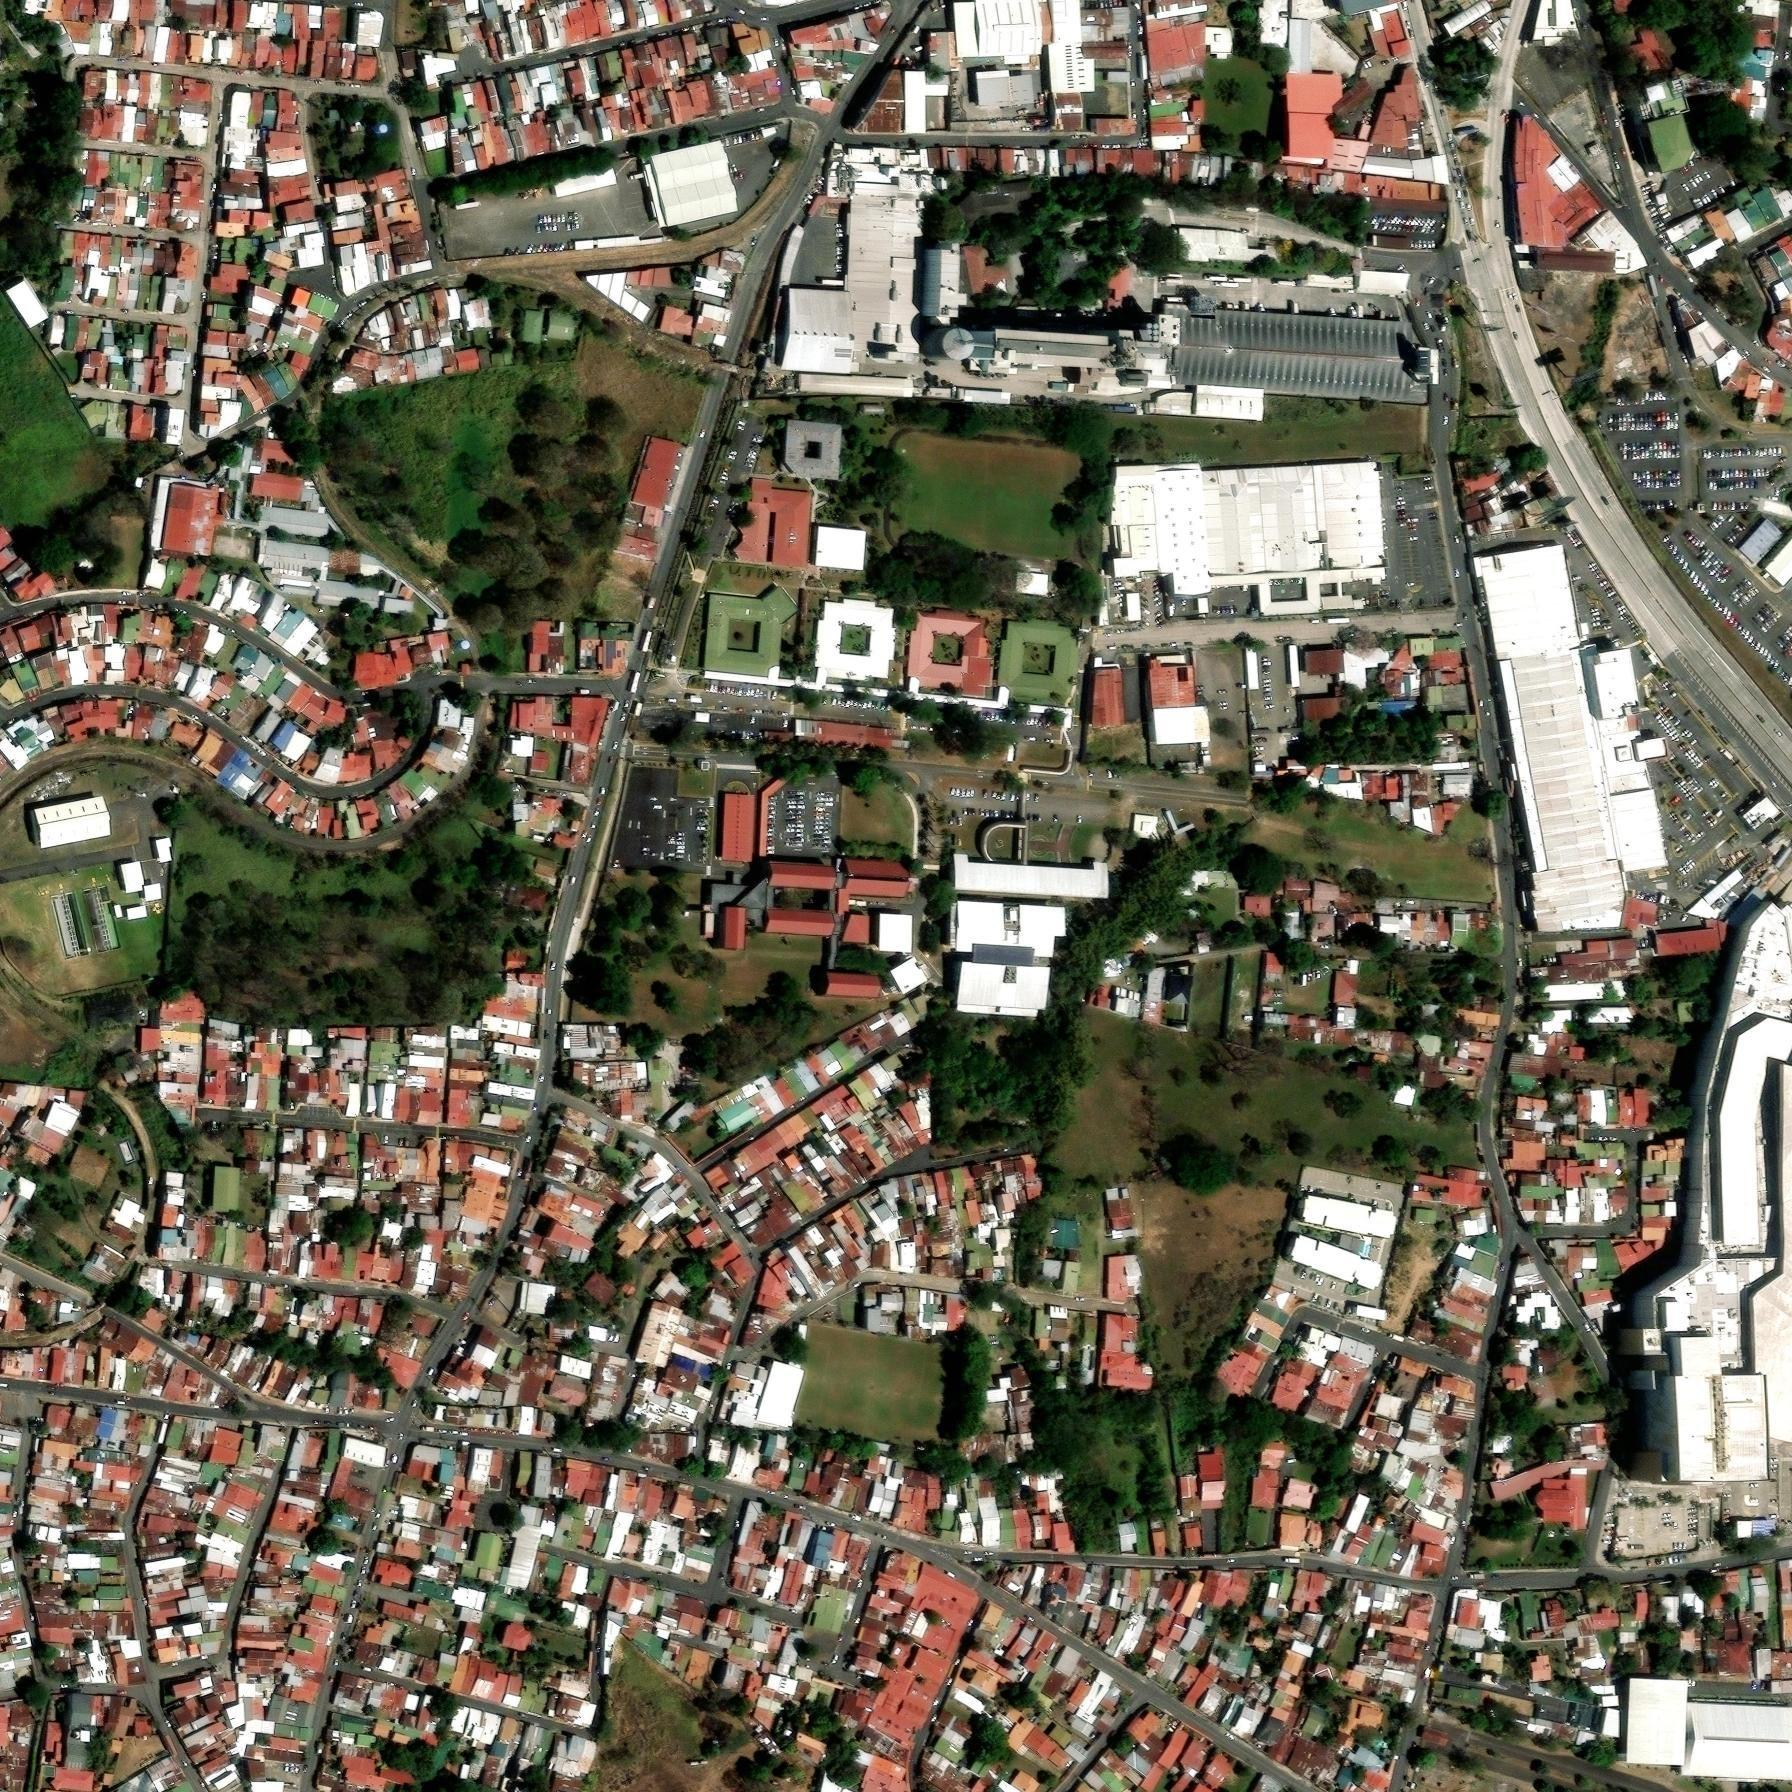
\includegraphics[width=0.85\textwidth]{figuras/satelital_campus_z18.jpg}
\caption{Imagen satelital del campus UTN Villa Bonita (Esri World Imagery, nivel 18, 0,59~m por píxel, descargada el 1/11/2026). El CAA-TEC es el edificio blanco girado junto a los techos rojos; el parqueo norte está entre la calle interna y la plaza del arco.}
\label{fig:satelital}
\end{figure}

\textbf{Por qué este sitio.} Es el mismo campus del Proyecto~2, así que se conocen el transformador, la medición, la malla de tierra y la ruta de la acometida existente, verificados en sitio. El parqueo ya existe y tiene una franja verde al sur, donde caben la isla de cargadores y la celda eléctrica sin quitar circulación. Está a menos de 120~m del transformador y la ruta del alimentador evita edificios y árboles (lámina VE-00).

{\small
\begin{longtable}{L{3.3cm}L{5.4cm}L{6.3cm}}
\caption{Supuestos de diseño (marcados con \supuesto{} en el texto).}\label{tab:supuestos}\\
\toprule
\textbf{Dato} & \textbf{Valor adoptado y fundamento} & \textbf{Efecto si el valor real difiere}\\
\midrule\endfirsthead
\toprule
\textbf{Dato} & \textbf{Valor adoptado y fundamento} & \textbf{Efecto si el valor real difiere}\\
\midrule\endhead
Capacidad remanente del transformador 119688 & $\ge$ 100~kVA. El CAA demanda unos 110~kVA (P2); el resto de las cargas de la UTN se desconoce & Si es menor, el EMS puede bajar el límite (por ejemplo, a 40~kW) o el ICE cambia el transformador. Lo define el estudio de capacidad.\\
Impedancia del transformador & 5,75\,\%, X/R = 5 (valor típico de 750~kVA) & Con 4,5\,\%, la corriente de falla sube a unos 20~kA, todavía menor que los 35~kA de IP-VE.\\
Posición del nicho y longitud del alimentador & Según E01; ruta medida de unos 111~m; se adoptan 120~m & Con 150~m, la caída sube a 1,9\,\% con \#3/0; sigue cumpliendo.\\
Impedancia de T-VE & 4,5\,\% & Corriente de falla en TD-AC de 2,8~kA o menos, frente a 10~kA de capacidad.\\
Temperatura ambiente & 31--35~°C (factor 0,96), como en P2 & Conservador para el Valle Central.\\
Eficiencias de carga & CA red--batería 0,90; cargador CC 0,95; vehículo en CC 0,97 & $\pm$5\,\% en energía y tiempo.\\
Curvas de aceptación en CC & Forma típica con el máximo del fabricante (\texttt{calc/carga.py}) & El tiempo del 20 al 80\,\% depende poco de ellas porque DC-1 limita a 60~kW.\\
Capacidades útiles & Leaf 39~kWh y Model Y 75~kWh (no publicadas como ``útiles'') & Proporcional en energía y tiempo.\\
Escenario de uso & 14 sesiones por día lectivo, 250 días lectivos y 115 días con 30\,\% del uso & Con la mitad del uso, el costo por kWh sube (sección~\ref{sec:economia}).\\
Espacios & 2,50~m $\times$ 5,00~m como base, ensanchados a 2,6--2,8~m; accesible de 3,30~m $\times$ 5,00~m & Confirmar con el reglamento de construcciones y el de la Ley 7600.\\
Precios sin cotización & Estimaciones de mercado (Cuadro~\ref{tab:bom}); tipo de cambio de ₡505/USD & El presupuesto puede variar $\pm$20\,\%.\\
Iluminación & 50~lx medios en la zona de conexión & Confirmar con INTE N121.\\
\bottomrule
\end{longtable}}

\subsection{Criterios de diseño}
\begin{enumerate}[leftmargin=1.2cm]
\item Atender la flota real del país sin depender de adaptadores no aprobados: J1772, GB/T, CCS1 y CHAdeMO.
\item Dar carga lenta en CA a quien permanece varias horas (la mayoría de los usuarios del campus) y carga rápida en CC a visitantes y a quien necesita autonomía inmediata.
\item Usar un servicio propio con medición independiente del CAA, para aplicar la tarifa correcta y, si se decide, vender el servicio (Ley 10937).
\item Seleccionar equipos listados (UL) cuando existan. Si no existen (GB/T), documentar la evaluación de la conformidad y agregar protección.
\item Considerar todas las cargas como continuas (125\,\%), con caída de tensión de 3\,\% o menos por tramo y de 5\,\% o menos en total.
\item Limitar la demanda con un EMS para reducir el cargo por demanda y el riesgo de capacidad.
\item Dejar previstos dos puntos de CA más y un segundo cargador de CC (ducto de reserva y espacios libres).
\end{enumerate}

\subsection{Puntos de carga: cantidad, tipo, potencia y ubicación}
\begin{table}[H]
\centering\small
\caption{Puntos de carga de la estación.}\label{tab:puntos}
\begin{tabularx}{\textwidth}{L{1.3cm}L{1.1cm}L{2.6cm}L{2.2cm}L{2.0cm}Y}
\toprule
\textbf{Punto} & \textbf{Espacio} & \textbf{Tipo y potencia} & \textbf{Conector} & \textbf{Equipo} & \textbf{Vehículos compatibles y justificación}\\
\midrule
AC-1 & P1 (accesible) & Modo 3, 208~V, 40~A, 8,3~kW & J1772 (Tipo 1) & Autel AC Elite & Leaf, Ioniq 5, F-150 y Tesla con adaptador. Espacio accesible (Ley 7600).\\
AC-2 & P2 & Modo 3, 208~V, 40~A, 8,3~kW & J1772 & Autel AC Elite & Igual que AC-1.\\
AC-3 & P3 & Modo 3, 208~V, 32~A, 6,7~kW & GB/T CA & MDAC 132EN K & BYD (CR) y otros GB/T. No hay alternativa en CC dentro de la estación.\\
AC-4 & P4 & Modo 3, 208~V, 32~A, 6,7~kW & GB/T CA & MDAC 132EN K & Igual que AC-3.\\
DC-1 & P5 y P6 & Modo 4, 60~kW (30 + 30~kW) & CCS1 (P5) y CHAdeMO (P6) & Autel DC Fast 60~kW & Ioniq 5, F-150, Tesla con adaptador CCS1 (P5); Leaf (P6).\\
\bottomrule
\end{tabularx}
\end{table}

La lámina VE-00 (Fig.~\ref{fig:ve00}) ubica la estación en el campus, junto con el transformador del ICE y la ruta del alimentador. La lámina VE-01 (Fig.~\ref{fig:ve01}) muestra a escala 1:100 los espacios, los cargadores, la celda eléctrica, los recorridos de las canalizaciones, los accesos, las cotas y la leyenda de símbolos.

\lamina{laminas/VE-00.pdf}{Lámina VE-00 (A3): plano general de ubicación sobre la imagen satelital del campus.}{fig:ve00}
\lamina{laminas/VE-01.pdf}{Lámina VE-01 (A3): planta de la estación a escala 1:100, con espacios, equipos, canalizaciones, accesos, cotas y leyenda.}{fig:ve01}

\subsection{Diagrama unifilar}
La lámina VE-02 (Fig.~\ref{fig:ve02}) muestra el sistema desde los bornes del transformador del ICE hasta cada cargador: tensiones, fases, circuitos, conductores, protecciones, medios de desconexión, medición (ICE y EMS) y puesta a tierra.

\lamina{laminas/VE-02.pdf}{Lámina VE-02 (A3): diagrama unifilar de la estación.}{fig:ve02}

\subsection{Energía, potencia efectiva y tiempo de carga}
\label{sec:calc_carga}
\textbf{Procedimiento} (\texttt{calc/carga.py}). La potencia que llega a la batería en cada instante es el mínimo de tres límites, afectado por las pérdidas:
\begin{equation}
P_{bat}(SOC)=\eta\cdot\min\Big(\underbrace{P_{EVSE}}_{\text{cargador}},\;\underbrace{P_{veh}(SOC)}_{\text{vehículo}},\;\underbrace{V_{sum}\,I_{max}}_{\text{suministro}}\Big)
\end{equation}
\begin{itemize}
\item En CA, $P_{veh}$ es la potencia del cargador a bordo (constante hasta el 95\,\% de SOC, con reducción posterior por el balanceo de celdas).
\item En CC, $P_{veh}$ es la curva de aceptación del vehículo, que baja con el SOC. Además, CHAdeMO está limitado a 125~A.
\end{itemize}
El tiempo se obtiene integrando el SOC sin suponer potencia constante, $t=\int_{SOC_0}^{SOC_1}E_u\,dSOC/P_{bat}(SOC)$, y la energía tomada de la red es $E_{red}=\int P_{red}\,dt$. Se distinguen la potencia en kW y la energía en kWh.

\textbf{Ejemplo manual (BYD Dolphin en AC-3, del 20 al 80\,\%).}
\begin{itemize}
\item Límites: el EVSE da $208\times 32=\SI{6.66}{\kilo\watt}$; el OBC, \SI{6.6}{\kilo\watt}. Gobierna el OBC: $P_{red}=\SI{6.6}{\kilo\watt}$ y $P_{bat}=0{,}9\times 6{,}6=\SI{5.94}{\kilo\watt}$.
\item Energía a la batería: $\Delta E=0{,}6\times 44{,}9=\SI{26.9}{\kilo\watt\hour}$.
\item Resultado: $t=26{,}9/5{,}94=\SI{4.54}{\hour}$ (4~h~32~min) y $E_{red}=26{,}9/0{,}9=\SI{29.9}{\kilo\watt\hour}$, que coinciden con el programa.
\end{itemize}
\textbf{Efecto de la tensión de 208~V.} Con 40~A, el Ioniq~5 recibe \SI{8.3}{\kilo\watt} a 208~V, frente a \SI{9.6}{\kilo\watt} a 240~V: el tiempo del 20 al 80\,\% pasa de unas 5~h~22~min a 6~h~12~min. Se acepta porque la permanencia típica en el campus supera las 6~h, y porque el servicio de la UTN es trifásico.

\begin{table}[H]
\centering\small
\caption{Energía, potencia y tiempo de carga del 20 al 80\,\% de SOC (\texttt{calc/carga\_out.txt}).}\label{tab:tiempos}
\begin{tabularx}{\textwidth}{L{3.6cm}L{3.7cm}rrrrY}
\toprule
\textbf{Vehículo} & \textbf{Punto} & \textbf{$E_{bat}$ (kWh)} & \textbf{$E_{red}$ (kWh)} & \textbf{$\bar P_{bat}$ (kW)} & \textbf{$P_{red,max}$ (kW)} & \textbf{Tiempo}\\
\midrule
BYD Dolphin & AC-3/AC-4 (GB/T) & 26,9 & 29,9 & 5,9 & 6,6 & 4~h~32~min\\
Nissan Leaf & AC-1/AC-2 & 23,4 & 26,0 & 5,9 & 6,6 & 3~h~56~min\\
Nissan Leaf & DC-1 CHAdeMO (solo) & 23,4 & 25,4 & 36,0 & 47,6 & 39~min\\
Nissan Leaf & DC-1 compartido & 23,4 & 25,4 & 28,3 & 31,6 & 50~min\\
Hyundai Ioniq 5 & AC-1/AC-2 & 46,4 & 51,6 & 7,5 & 8,3 & 6~h~12~min\\
Hyundai Ioniq 5 & DC-1 CCS1 (solo) & 46,4 & 50,4 & 58,2 & 63,2 & 48~min\\
Hyundai Ioniq 5 & DC-1 compartido & 46,4 & 50,4 & 29,1 & 31,6 & 1~h~36~min\\
Tesla Model Y & AC-1/AC-2 (adaptador) & 45,0 & 50,0 & 7,5 & 8,3 & 6~h~01~min\\
Tesla Model Y & DC-1 CCS1 (adaptador) & 45,0 & 48,8 & 58,2 & 63,2 & 46~min\\
F-150 Lightning ER & AC-1/AC-2 & 78,6 & 87,3 & 7,5 & 8,3 & 10~h~30~min\\
F-150 Lightning ER & DC-1 CCS1 (solo) & 78,6 & 85,3 & 58,2 & 63,2 & 1~h~21~min\\
F-150 Lightning ER & DC-1 compartido & 78,6 & 85,3 & 29,1 & 31,6 & 2~h~42~min\\
\bottomrule
\end{tabularx}
\end{table}

\textbf{Lectura de los resultados.}
\begin{itemize}
\item En CA el límite lo pone el OBC en el Leaf y el Dolphin (6,6~kW) y el EVSE a 208~V en los vehículos de 10,9 a 19,2~kW.
\item En CC, el límite de 60~kW de DC-1 gobierna los vehículos con curvas altas (Ioniq 5, F-150, Model Y), mientras que el Leaf queda limitado por su propia curva y por CHAdeMO.
\item Cargar del 20 al 100\,\% en CC es ineficiente: el Leaf tarda 1~h~27~min (frente a 39~min hasta el 80\,\%) y el Model Y, 1~h~20~min. Por eso DC-1 se configura con un tope del 80\,\% para usuarios en espera.
\item La F-150 necesita 10~h~30~min en CA para recibir 78,6~kWh: para una pickup de batería grande en uso diario, el punto adecuado es DC-1.
\end{itemize}

\textbf{Escenario de uso y energía anual.} Con 14 sesiones por día lectivo (Cuadro~\ref{tab:supuestos}), la estación entrega 521~kWh a las baterías y toma 572~kWh de la red por día. DC-1 queda ocupado unas 5~h al día. Al año son \textbf{162,8~MWh} (81,5 en CA y 81,3 en CC), unos 13\,560~kWh al mes.

\subsection{Conductores, canalizaciones y caída de tensión}
\label{sec:cond}
\textbf{Procedimiento} (\texttt{calc/electrico.py}):
\begin{enumerate}
\item Corriente de diseño: $I_d=1{,}25\,I_{max}$ (625.41, 215.2).
\item Interruptor: el valor normalizado igual o siguiente (240.6).
\item Conductor con ampacidad $I_z=\min(I_{90}\,k_T\,k_A,\;I_{75})\ge I_d$, protegido por el interruptor (240.4(B)).
\item EGC según la Tabla 250.122.
\item Caída de tensión con la impedancia eficaz de la Tabla 9: $\Delta V=k\,I\,L\,(R\cos\phi+X\sin\phi)$, con $k=\sqrt3$ en circuitos trifásicos y $k=2$ en monofásicos.
\end{enumerate}

\begin{table}[H]
\centering\small
\caption{Dimensionamiento de conductores, protecciones y canalizaciones.}\label{tab:conductores}
\footnotesize\setlength{\tabcolsep}{3pt}
\begin{tabular}{L{1.5cm}R{1.0cm}R{1.0cm}L{1.9cm}L{3.0cm}R{0.9cm}R{0.7cm}R{0.9cm}L{2.7cm}}
\toprule
\textbf{Circuito} & \textbf{$I_{max}$ (A)} & \textbf{1,25$I$ (A)} & \textbf{OCPD (A)} & \textbf{Conductores Cu THWN-2} & \textbf{$I_z$ (A)} & \textbf{L (m)} & \textbf{$\Delta V$ (\%)} & \textbf{Tubo PVC-40 (ocupación)}\\
\midrule
AL-VE & 146,2 & 182,8 & 200, 3P & 3\#3/0 + N\#4 + EGC\#6 & 200 & 120 & 1,54 & 3'' (12,9\,\%) + reserva\\
DC-1 & 91,0 & 113,8 & 125, 3P & 3\#1 + EGC\#6 & 130 & 8 & 0,13 & 1-1/2'' (26,2\,\%)\\
T-VE prim. & 54,1 & 67,7 & 70, 3P & 3\#4 + EGC\#8 & 85 & 3 & -- & 1''\\
T-VE sec. & 124,9 & -- & 125 (TD-AC) & 3\#1 + N\#1 + EGC\#6 & 130 & $\le$3 & 0,13 & 1-1/2''\\
AC-1, AC-2 & 40 & 50 & 50, 2P & 2\#6 + EGC\#10 c/u & 57,6 & 18 & 1,12 & 1'' (26,9\,\%, 2 circ.)\\
AC-3, AC-4 & 32 & 40 & 40, 2P + RCD B & 2\#8 + EGC\#10 c/u & 42,2 & 13 & 1,02 & 1'' (20,1\,\%, 2 circ.)\\
Alumbrado & 1,1 & 1,4 & 20, 1P 277~V & 2\#12 + EGC\#12 & 25 & 40 & $<$0,5 & 3/4'' (7,9\,\%)\\
\bottomrule
\end{tabular}
\end{table}

\begin{itemize}
\item \textbf{Alimentador:} se dimensionó con la capacidad nominal completa de T-VE (54,1~A) para dejar prevista la ampliación de CA: $1{,}25\times(91+54{,}1+1{,}1)=\SI{182.8}{\ampere}$. Con la carga instalada real (129,3~A), la caída es de 1,54\,\%. Con \#2/0 sería de 1,97\,\%, pero su ampacidad (175~A) queda por debajo de 182,8~A, así que se descarta.
\item \textbf{Caída total:} 1,68\,\% hasta DC-1 y 2,79\,\% en el peor ramal de CA, dentro del criterio de 5\,\%.
\item \textbf{Canalizaciones:} todas subterráneas a 600~mm, con ocupación de 40\,\% o menos. Se usan tubos de 3'' en el alimentador para facilitar el halado de 120~m, más un ducto de reserva para un segundo cargador de CC.
\item \textbf{Balance de fases en 208~V:} A = 92,3~A, B = 98,3~A, C = 70,8~A. La fase más cargada al 125\,\% da 122,9~A, menor que el principal de 125~A de TD-AC.
\end{itemize}

\subsection{Protecciones, puesta a tierra y medios de desconexión}
\label{sec:cc}
\begin{itemize}
\item \textbf{Sobrecorriente:} las del Cuadro~\ref{tab:conductores}.
  \begin{itemize}
  \item T-VE se protege solo en el primario con 125\,\% o menos (70~A $\ge$ 67,7~A, permitido por la nota~1 de la Tabla 450.3(B)).
  \item Los conductores del secundario, de 3~m o menos, terminan en el principal de 125~A de TD-AC (240.21(C)(2)).
  \end{itemize}
\item \textbf{Capacidad interruptiva:} se calculó con barra infinita y $Z$ = 5,75\,\% \supuesto{}.
  \begin{itemize}
  \item $I_{cc}=\SI{15.7}{\kilo\ampere}$ en los bornes del transformador: IP-VE es un PowerPact J de 35~kA. El interruptor existente del CAA es de 18~kA.
  \item \SI{5.8}{\kilo\ampere} en TD-VE (tablero de 14~kA o más).
  \item \SI{2.8}{\kilo\ampere} en TD-AC (QO de 10~kA).
  \item DC-1 tiene un SCCR de 65~kA o más.
  \end{itemize}
  Los valores se rotulan en TD-VE (110.24).
\item \textbf{Falla a tierra y corrientes residuales:}
  \begin{itemize}
  \item AC-1/AC-2 llevan un CCID de 20~mA integrado (UL 2231).
  \item DC-1 tiene monitoreo de aislamiento (IMD), detección de falla a tierra y botón de emergencia.
  \item AC-3/AC-4 llevan, además de su protección interna contra fugas, un \textbf{diferencial tipo~B de 30~mA} aguas arriba. Así detectan fallas con componente continua que un diferencial tipo~A no ve (IEC 60364-7-722), y quedan cubiertos aunque no tengan listado UL.
  \end{itemize}
\item \textbf{Sobretensiones:} SPD tipo~1 en TD-VE, tipo~2 en TD-AC y los SPD internos de los cargadores.
\item \textbf{Puesta a tierra:} electrodo propio de dos varillas (250.32, 250.53) con GEC \#6. T-VE es un sistema derivado separadamente con puente N--T propio (250.30). En TD-VE el neutro y la tierra van separados. EGC continuo y unión de las partes metálicas (VE-03, D4).
\item \textbf{Desconexión:}
  \begin{itemize}
  \item IP-VE: desconectador del servicio en el nicho, rotulado.
  \item Principal de TD-VE con disparo en derivación, accionado por EPO-1 o EPO-2 (desenergiza toda la estación).
  \item Interruptor de DC-1 bloqueable en abierto (625.43).
  \item Interruptores de los ramales en TD-AC, a la vista de los pedestales.
  \end{itemize}
\item \textbf{Coordinación con las protecciones integradas:}
  \begin{itemize}
  \item Ante una sobrecarga o falla del lado del vehículo, actúan primero las protecciones internas del EVSE: los relés que abren el contactor y el CCID.
  \item Una falla interna del equipo la despeja su interruptor de ramal: 40/50~A frente a 125~A en TD-AC, y 125~A frente a 200~A en TD-VE.
  \end{itemize}
  La relación de corrientes nominales entre niveles es de 1,6 o más, lo que da selectividad en la zona de sobrecarga. En la zona instantánea no se garantiza, y el NEC no la exige en este tipo de instalación.
\end{itemize}

\subsection{Detalles de conexión y montaje}
La lámina VE-03 (Fig.~\ref{fig:ve03}) reúne los detalles:
\begin{itemize}
\item D1: pedestal de CA, con conector a 0,9--1,2~m, gestor de cable, dado de anclaje y bolardo.
\item D2: sección de la zanja, a 600~mm, con arena, cinta de advertencia y ducto de reserva.
\item D3: base de DC-1.
\item D4: puesta a tierra.
\item D5: rotulación (NEC 110.21, 110.24, 625.43, INTE N120 y Ley 7600).
\item D6: emergencia y mantenimiento.
\end{itemize}
Contra el agua, todo va sobre bases elevadas, con entrada de tubos por abajo y sellada. Contra el polvo y la corrosión, se usan equipos NEMA 3R/4 o IP54 y herrajes inoxidables. Contra los impactos, bolardos y topes. Los cables y conectores se manejan con gestores de cable y fundas.

\lamina{laminas/VE-03.pdf}{Lámina VE-03 (A3): detalles de montaje, zanja, puesta a tierra, rotulación, emergencia y mantenimiento.}{fig:ve03}

\subsection{Cuadro de cargas, cuadro de equipos y lista de materiales}
\begin{table}[H]
\centering\small
\caption{Cuadro de cargas (corriente máxima de entrada de cada equipo, NEC 625.42).}\label{tab:cargas}
\begin{tabularx}{\textwidth}{L{1.6cm}L{4.4cm}rrrrY}
\toprule
\textbf{Circuito} & \textbf{Carga} & \textbf{V} & \textbf{I (A)} & \textbf{kVA} & \textbf{Fases} & \textbf{Tablero / protección}\\
\midrule
DC-1 & Cargador rápido 60~kW & 480 & 91,0 & 75,7 & 3F & TD-VE, 3P 125~A\\
AC-1 & Cargador J1772 & 208 & 40 & 8,32 & A-B & TD-AC, 2P 50~A\\
AC-2 & Cargador J1772 & 208 & 40 & 8,32 & B-C & TD-AC, 2P 50~A\\
AC-3 & Cargador GB/T & 208 & 32 & 6,66 & C-A & TD-AC, 2P 40~A + RCD B\\
AC-4 & Cargador GB/T & 208 & 32 & 6,66 & A-B & TD-AC, 2P 40~A + RCD B\\
AUX & Tomacorriente, EMS, router, control & 120 & 8,3 & 1,00 & C & TD-AC, 1P 20~A\\
ILUM & 2 luminarias LED 150~W & 277 & 1,1 & 0,30 & -- & TD-VE, 1P 20~A\\
\midrule
\multicolumn{4}{l}{\textbf{Total instalado (sin EMS)}} & \textbf{107,0} & & demanda $\approx$ 94,5~kW\\
\multicolumn{4}{l}{\textbf{Límite con EMS (625.42)}} & & & 60~kW\\
\bottomrule
\end{tabularx}
\end{table}

\begin{table}[H]
\centering\small
\caption{Cuadro de equipos principales.}\label{tab:equipos}
\begin{tabularx}{\textwidth}{L{1.5cm}L{4.5cm}Y}
\toprule
\textbf{Código} & \textbf{Equipo (fabricante y modelo)} & \textbf{Especificación}\\
\midrule
DC-1 & Autel MaxiCharger DC Fast 60~kW, UF060A3001 & 480~V 3F, 91~A; CCS1 + CHAdeMO; UL 2202; NEMA 3R; OCPP\\
AC-1, AC-2 & Autel MaxiCharger AC Elite 50A, MC50AHS & 208~V, ajustado a 40~A; J1772 con 7,5~m; UL 2594; NEMA 4\\
AC-3, AC-4 & MDAC 132EN K, cabezal GB/T & 208~V entre fases, 32~A; GB/T; IP54; OCPP 1.6\\
T-VE & Transformador seco 45~kVA (Square D EE45T3H o equivalente) & 480$\Delta$--208Y/120~V; NEMA 3R; UL 1561\\
IP-VE & Schneider PowerPact JGL36200 en gabinete NEMA 3R & 200~A 3P, 480~V, 35~kA\\
TD-VE & Tablero 480Y/277~V, 225~A, principal de 200~A con disparo en derivación & NEMA 3R, 14~kA o más; SPD tipo 1\\
TD-AC & Square D QO, 208Y/120~V, 125~A, 24 espacios & NEMA 3R, 10~kA; SPD tipo 2\\
RCD-B & Diferencial tipo B 2P 40~A 30~mA & Para AC-3/AC-4\\
EMS & Controlador de gestión vía OCPP con TC en AL-VE & Límite de 60~kW\\
\bottomrule
\end{tabularx}
\end{table}

{\small
\begin{longtable}{L{1.4cm}L{7.4cm}rL{0.8cm}rrL{0.9cm}}
\caption{Lista de materiales y presupuesto referencial (USD, sin IVA, \texttt{calc/economico.py}). F = fuente del precio (Autel: tienda del fabricante, 1/11/2026; S: estimación de mercado).}\label{tab:bom}\\
\toprule
\textbf{Código} & \textbf{Descripción} & \textbf{Cant.} & \textbf{Ud.} & \textbf{P. unit.} & \textbf{Subtotal} & \textbf{F}\\
\midrule\endfirsthead
\toprule
\textbf{Código} & \textbf{Descripción} & \textbf{Cant.} & \textbf{Ud.} & \textbf{P. unit.} & \textbf{Subtotal} & \textbf{F}\\
\midrule\endhead
DC-1 & Autel MaxiCharger DC Fast 60~kW UL, CCS1 + CHAdeMO & 1 & u & 28\,000 & 28\,000 & S\\
AC-1/2 & Autel MaxiCharger AC Elite 50~A cableado, J1772 7,5~m & 2 & u & 639 & 1\,278 & Autel\\
AC-3/4 & Cargador CA GB/T 7~kW 32~A, IP54, OCPP 1.6 & 2 & u & 650 & 1\,300 & S\\
PED & Pedestal metálico doble con soporte de cable & 2 & u & 450 & 900 & S\\
RCD-B & Diferencial tipo B 2P 40~A 30~mA & 2 & u & 280 & 560 & S\\
T-VE & Transformador seco 45~kVA 480$\Delta$--208Y/120~V NEMA 3R & 1 & u & 5\,200 & 5\,200 & S\\
IP-VE & Interruptor 200~A 3P 35~kA en gabinete NEMA 3R & 1 & u & 2\,600 & 2\,600 & S\\
TD-VE & Tablero 480Y/277~V 225~A con principal de 200~A y disparo en derivación & 1 & u & 4\,800 & 4\,800 & S\\
INT-480 & Interruptores 3P 125~A, 3P 70~A y 1P 20~A 277~V & 1 & lote & 1\,620 & 1\,620 & S\\
TD-AC & Tablero QO 125~A 24 espacios con interruptores & 1 & u & 1\,000 & 1\,000 & S\\
SPD & Supresores tipo 1 y tipo 2 (UL 1449) & 1 & lote & 1\,300 & 1\,300 & S\\
EPO & Botones de paro de emergencia con rótulo & 2 & u & 250 & 500 & S\\
C-3/0 & Cu THWN-2 3/0 (3 $\times$ 126~m) & 378 & m & 14,0 & 5\,292 & S\\
C-4/6 & Cu THWN-2 \#4 (neutro) y \#6 (EGC) & 252 & m & 3,8 & 958 & S\\
C-RAM & Conductores de ramales & 1 & lote & 950 & 950 & S\\
PVC-3 & PVC cédula 40 de 3'' (alimentador + reserva) & 252 & m & 6,5 & 1\,638 & S\\
PVC-R & PVC de 3/4'' a 1-1/2'' y accesorios & 1 & lote & 650 & 650 & S\\
ZANJA & Zanja de 0,6~m con corte y reposición de asfalto & 125 & m & 45 & 5\,625 & S\\
REG & Registros de 60$\times$60~cm con tapa de tránsito & 5 & u & 350 & 1\,750 & S\\
BASES & Bases de concreto y anclajes & 1 & lote & 2\,500 & 2\,500 & S\\
BOL & Bolardos de acero rellenos de concreto & 10 & u & 180 & 1\,800 & S\\
TOPE & Topes de rueda & 6 & u & 60 & 360 & S\\
LUM & Postes de 6~m con luminaria LED de 150~W & 2 & u & 1\,400 & 2\,800 & S\\
PAT & Puesta a tierra (varillas, \#4 desnudo, soldadura) & 1 & lote & 600 & 600 & S\\
SEÑAL & Demarcación y rótulos (INTE N120, Ley 7600, NEC) & 1 & lote & 1\,200 & 1\,200 & S\\
MED & Medición indirecta del ICE y aporte de conexión & 1 & lote & 2\,500 & 2\,500 & S\\
MO & Mano de obra eléctrica y civil & 1 & lote & 9\,000 & 9\,000 & S\\
PEM & Puesta en marcha, OCPP, módem 4G, capacitación & 1 & lote & 1\,500 & 1\,500 & S\\
ING & Diseño, planos, CFIA, dirección técnica y permisos & 1 & lote & 5\,000 & 5\,000 & S\\
\midrule
 & \textbf{Subtotal} & & & & \textbf{93\,181} & \\
 & Imprevistos (10\,\%) & & & & 9\,318 & \\
 & \textbf{Total (unos ₡51,8 millones a ₡505/USD)} & & & & \textbf{102\,499} & \\
\bottomrule
\end{longtable}}

\subsection{Consumo y costo de operación}
\label{sec:economia}
Con 162,8~MWh al año y la demanda máxima mensual de la estación, el costo anual (\texttt{calc/economico.py}) incluye la energía, la demanda (12 meses) y la operación y mantenimiento: USD~3300 al año, que cubren el contrato de DC-1, el mantenimiento de la obra, la plataforma OCPP, la conectividad y la póliza de la Ley 10937.

\begin{table}[H]
\centering\small
\caption{Costo anual de operación según la tarifa y la gestión de carga (millones de colones, sin impuestos).}\label{tab:operacion}
\begin{tabularx}{\textwidth}{L{3.2cm}L{2.0cm}rrrrY}
\toprule
\textbf{Tarifa ICE 2026} & \textbf{Gestión} & \textbf{Energía} & \textbf{Demanda} & \textbf{O\&M} & \textbf{Total} & \textbf{₡/kWh (peso de la demanda)}\\
\midrule
T-CO & sin EMS (94,5~kW) & 9,71 & 11,18 & 1,67 & 22,56 & 138,6 (54\,\%)\\
T-CO & EMS 60~kW & 9,71 & 7,10 & 1,67 & 18,48 & 113,5 (42\,\%)\\
T-CS & sin EMS & 8,25 & 9,50 & 1,67 & 19,42 & 119,3 (54\,\%)\\
T-CS & EMS 60~kW & 8,25 & 6,04 & 1,67 & 15,96 & 98,0 (42\,\%)\\
\bottomrule
\end{tabularx}
\end{table}

El cargo por demanda es tan grande como el de energía porque DC-1 concentra hasta \SI{63}{\kilo\watt} en pocas horas al mes. El EMS reduce el costo anual entre ₡3,5 y ₡4,1 millones, con un costo casi nulo porque solo es configuración OCPP y un TC. Con precios iguales a los de la red pública (₡99,70/kWh en CA y ₡141/min en CC), los ingresos serían de unos ₡20,2 millones al año. La sección~\ref{sec:viabilidad} analiza el retorno.

\subsection{Funciones bidireccionales, fotovoltaica y almacenamiento}
La propuesta no incorpora carga entre vehículos, funciones bidireccionales, generación FV ni almacenamiento (sección~\ref{sec:bidir}), por lo que no requiere esquemas de flujo de energía adicionales. La razón principal es regulatoria: no hay un marco V2G aplicable ni equipos bidireccionales certificados disponibles. Hay además una razón económica: el cargo por demanda se controla más barato con el EMS que con una batería.

\subsection{Emergencia, mantenimiento, ampliación y cambios en la instalación existente}
\label{sec:ampliacion}
\begin{itemize}
\item \textbf{Emergencia:} dos EPO que abren TD-VE, el botón propio de DC-1, el procedimiento rotulado (VE-03, D6), un extintor y acceso libre para Bomberos por la calle interna. Ante un incendio de batería, el protocolo es desenergizar, aislar la zona y esperar a Bomberos.
\item \textbf{Mantenimiento:} el plan preventivo mensual, semestral y anual de VE-03. Para disponibilidad de repuestos se elige un solo fabricante principal (Autel) para los equipos UL, y se mantienen en sitio un conector J1772 y un cable CCS1.
\item \textbf{Ampliación:}
  \begin{itemize}
  \item T-VE (45~kVA, 69\,\% de uso) y TD-AC (dos espacios 2P de reserva) admiten dos puntos de CA más.
  \item TD-VE tiene un espacio 3P de reserva y existe un ducto de 3'' de reserva para un segundo cargador de CC. Ese cargador requiere aumentar IP-VE y el alimentador, o reducir la potencia con el EMS, y un nuevo estudio de capacidad del ICE.
  \item Una batería estacionaria o un sistema FV en el servicio de la estación reducirían la demanda facturada.
  \end{itemize}
\item \textbf{Cambios en la instalación existente:} la única intervención sobre la infraestructura actual es la conexión del servicio nuevo en el nicho del transformador 119688 (medición y IP-VE), que hace o autoriza el ICE. No se modifican el servicio, el TS-01 ni el TP del CAA. En el parqueo se pierden seis espacios de uso general, que pasan a ser exclusivos para VE, y se construye la isla sobre la franja verde existente.
\end{itemize}

% =====================================================================
\section{Análisis de la propuesta y de su viabilidad}
\label{sec:analisis}

\subsection{Por qué esta modalidad, estos equipos y esta potencia}
\begin{itemize}
\item \textbf{Modalidad mixta (CA + CC).} En un campus la mayoría de los usuarios estacionan de 4 a 9~horas. En ese tiempo, 6,6 a 8,3~kW alcanzan para recuperar del 20 al 80\,\% de casi cualquier automóvil o SUV (4 a 6~h, Cuadro~\ref{tab:tiempos}). La carga en CA es la de menor costo por punto (unos USD~900--1200 por punto en equipos, frente a USD~28\,000 de DC-1) y la de menor demanda. DC-1 atiende a visitantes, pickups de batería grande y usuarios con urgencia, y es el único medio de carga rápida para CHAdeMO en la zona.
\item \textbf{60~kW y no 120~kW.} Con 60~kW, un vehículo pasa del 20 al 80\,\% en 40--80~min. La corriente (91~A) cabe en un alimentador de 200~A desde el transformador existente. Un ABB Terra 124 de 120~kW tomaría 153~A, exigiría un servicio de 250~A o más y duplicaría el cargo por demanda, para un ahorro de tiempo que en un campus no es crítico.
\item \textbf{Conectores.} Se cubren los cuatro grupos de la flota real: J1772/CCS1, CHAdeMO, GB/T y NACS con adaptador aprobado. Esto se decidió a partir de la verificación por versión y mercado (sección~\ref{sec:compat}), no de la forma del conector.
\end{itemize}

\subsection{Ventajas y limitaciones frente a otras alternativas; estación residencial frente a pública}
{\small
\begin{longtable}{L{3.2cm}L{5.6cm}L{6.2cm}}
\caption{Ventajas y limitaciones de la propuesta frente a otras alternativas.}\label{tab:ventajas}\\
\toprule
\textbf{Alternativa} & \textbf{Ventaja de la propuesta} & \textbf{Limitación de la propuesta}\\
\midrule\endfirsthead
\toprule
\textbf{Alternativa} & \textbf{Ventaja} & \textbf{Limitación}\\
\midrule\endhead
Solo CA (Nivel 2) & Atiende pickups, visitantes y CHAdeMO en menos de 1~h & Más inversión (DC-1 es el 30\,\% del presupuesto) y cargo por demanda\\
Solo CC rápida & Atiende a muchos usuarios que permanecen varias horas, a bajo costo, y a la flota GB/T & Un solo cargador rápido: en horas pico hay espera, y con dos vehículos la potencia baja a 30 + 30~kW\\
Tomacorrientes de 120~V (Modo 2) & 4 a 6 veces más potencia; autenticación, medición y protección propia & Costo de los EVSE\\
Cargadores de pared domésticos sin red & Gestión, cobro y EMS por OCPP & Requiere conectividad y plataforma\\
CC de 120--180~kW & Menor demanda y alimentador existente suficiente & Más tiempo para las baterías grandes\\
Cargador CC con GB/T (IEC, 400~V) & Equipo listado UL a 480~V sin transformador & Los GB/T solo cargan en CA dentro de la estación\\
V2G/FV/almacenamiento & Menor complejidad regulatoria y de costo & No aprovecha FV ni reduce la demanda con una batería\\
\bottomrule
\end{longtable}}

\textbf{Estación residencial frente a pública.}
\begin{itemize}
\item \textbf{Residencial:} un solo usuario y un solo vehículo. Basta un wallbox de 7--10~kW en un circuito de 240~V del servicio monofásico, se mide con el medidor de la casa (tarifa residencial), no hay autenticación, cobro ni accesibilidad, y el trámite es el de una ampliación de la instalación interna.
\item \textbf{Pública:} multiusuario y flota mixta. Exige varios conectores, autenticación, medición por sesión, un EMS, servicio trifásico (208 o 480~V), medición propia, accesibilidad (Ley 7600), señalización, protección contra impactos, paros de emergencia y alumbrado. Si se vende la energía, entran la Ley 10937 y ARESEP (póliza, canon y tarifa). Por eso el costo por punto es mucho mayor.
\end{itemize}

\subsection{Cómo se aplicaron las normas en el diseño}
\begin{table}[H]
\centering\small
\caption{Matriz de cumplimiento: requisito, medida de diseño y evidencia.}\label{tab:cumplimiento}
\begin{tabularx}{\textwidth}{L{4.0cm}YL{2.6cm}}
\toprule
\textbf{Requisito (fuente)} & \textbf{Medida aplicada} & \textbf{Evidencia}\\
\midrule
Ley 9518 / Ley 10937 (art. 31--32) & Servicio y medidor propios, medición por sesión (OCPP), póliza de responsabilidad civil y consulta previa al ICE & Secc.~\ref{sec:ley9518}, VE-02\\
Reglamento de la Ley 9518: INTE/IEC 61851 & Equipos Modo 3 y Modo 4 conformes con la serie 61851 & Cuadro~\ref{tab:cargadores}\\
RTCR 458 / NEC 625 & Circuitos individuales, 125\,\%, desconexión bloqueable, CCID/IMD, cable de 7,5~m o menos & Cuadro~\ref{tab:nec}, VE-02\\
RTCR 458 art. 5.3 & Listado UL o certificado IEC/GB evaluado, más RCD tipo B & Secc.~\ref{sec:seleccion}\\
NEC 110.9/110.10/110.24 & Capacidades interruptivas mayores que la $I_{cc}$, rotuladas & Secc.~\ref{sec:cc}\\
NEC 110.26 & 1,10~m frente a los tableros & VE-01\\
NEC 250 & Electrodo propio, sistema derivado, EGC y uniones & VE-02, VE-03 D4\\
NEC 300.5 & Tubería a 600~mm con cinta de advertencia & VE-03 D2\\
INTE N121 (instalación, conectores, seguridad, información, estacionamiento, iluminación) & Los seis ejes cubiertos; valores numéricos por confirmar & VE-01, VE-03\\
INTE N120 & Identificador de compatibilidad en cada manguera & VE-03 D5\\
ICE / ARESEP & Solicitud de servicio, estudio de capacidad, medición indirecta, tarifa T-CO o T-CS & Secc.~\ref{sec:distribuidora}\\
Ley 7600 & Espacio accesible con franja, ruta accesible, alcance de 0,9--1,2~m & VE-01, VE-03 D1\\
RNPCI / Bomberos & EPO, extintor, acceso del camión, protocolo de baterías & VE-03 D6\\
CFIA / Municipalidad & Planos firmados (APC), dirección técnica, declaración jurada, permiso municipal & Secc.~\ref{sec:tramites}\\
\bottomrule
\end{tabularx}
\end{table}

\subsection{Viabilidad técnica, económica, de operación y de expansión}
\label{sec:viabilidad}
\begin{itemize}
\item \textbf{Técnica: viable.}
  \begin{itemize}
  \item Todos los equipos se pueden conseguir en el mercado.
  \item Los cálculos cumplen con margen: alimentador al 91\,\% de su ampacidad, caídas de 2,8\,\% o menos y capacidades interruptivas con 2,2 a 3,6 veces de margen.
  \item La condición crítica externa es la capacidad del transformador 119688, que debe confirmar el ICE. Con el EMS se puede adaptar a una capacidad menor.
  \end{itemize}
\item \textbf{Costo inicial:} USD~102\,500, de los cuales el 44\,\% son equipos principales y el resto obra civil, alimentador, mano de obra e ingeniería. El alimentador de 120~m y la zanja suman unos USD~13\,500. Ubicar la estación más cerca del transformador lo reduciría, pero no hay parqueo junto al nicho.
\item \textbf{Operación:} entre ₡98 y ₡139 por kWh, según la tarifa y el uso del EMS (Cuadro~\ref{tab:operacion}).
\item \textbf{Retorno simple, vendiendo a los precios de la red pública:}
  \begin{itemize}
  \item T-CS con EMS: unos 12 años; precio de equilibrio de ₡145/kWh a 10 años con una tasa del 8\,\%.
  \item T-CO con EMS: unos 30 años (₡161/kWh).
  \item Sin EMS no se recupera.
  \item Con la mitad del uso supuesto no se recupera en ningún escenario.
  \item Una fase inicial solo con CA tampoco se paga con ₡99,70/kWh: el ingreso por kWh en CA es bajo frente a la demanda y la inversión común.
  \end{itemize}
  En conclusión, \textbf{como negocio no es viable con los precios de referencia}, mientras que \textbf{como servicio institucional sí lo es}. El costo de operación de unos ₡98/kWh (T-CS con EMS) es parecido al precio público de CA, y la inversión se justifica como infraestructura de movilidad sostenible.
\item \textbf{Mantenimiento y repuestos:}
  \begin{itemize}
  \item Para los equipos UL, un fabricante principal (Autel) con garantía de 2 a 3 años, representación regional y repuestos de cables y conectores en sitio.
  \item El riesgo mayor está en los equipos GB/T, que tienen soporte local incierto. Se mitiga con una garantía exigida por contrato o con el uso del cargador que entrega BYD.
  \end{itemize}
\item \textbf{Expansión:} los dos puntos de CA adicionales son inmediatos (T-VE y TD-AC tienen reserva). Un segundo cargador de CC usaría el ducto de reserva, pero requiere un nuevo estudio de capacidad.
\end{itemize}

\subsection{Riesgos y medidas de mitigación}
{\small
\begin{longtable}{L{2.2cm}L{5.4cm}L{7.4cm}}
\caption{Riesgos y medidas propuestas.}\label{tab:riesgos}\\
\toprule
\textbf{Tipo} & \textbf{Riesgo} & \textbf{Medida}\\
\midrule\endfirsthead
\toprule
\textbf{Tipo} & \textbf{Riesgo} & \textbf{Medida}\\
\midrule\endhead
Eléctrico & Contacto con partes energizadas, cable dañado, falla a tierra en el vehículo & EVSE listados con CCID e IMD, RCD tipo B en los equipos IEC, EGC continuo, desconexión bloqueable, inspección mensual de cables y EPO\\
Eléctrico & Arco eléctrico al operar tableros de 480~V & Rótulo de riesgo de arco (110.16), espacio de trabajo y trabajo desenergizado con bloqueo y etiquetado\\
Incendio & Sobrecalentamiento de conexiones o incendio de una batería & Conductores al 125\,\%, termografía semestral, extintor, separación de la celda y de los vehículos, EPO y protocolo para Bomberos\\
Incendio & Adaptadores no aprobados & Rótulos que los prohíben (secc.~\ref{sec:compat}); el diseño no los necesita\\
Ambiental & Lluvia, inundación local, rayos, corrosión & Bases elevadas, NEMA 3R/4 o IP54, SPD tipo 1 y tipo 2, herrajes inoxidables\\
Ambiental & Disposición de equipos al final de su vida & Retiro por el proveedor según el manejo de residuos electrónicos\\
Circulación & Choque de vehículos con los equipos & Bolardos, topes de rueda, isla elevada y celda fuera de la zona de rodamiento\\
Circulación & Cables en el piso y tropiezos & Gestores de cable y espacios de 2,6--2,8~m\\
Circulación & Ocupación de espacios por vehículos que no cargan & Señalización, tiempo máximo y control por la aplicación\\
Regulatorio & Cambio de requisitos por el reglamento del MINAE (dic. 2026) y las tarifas de ARESEP & Revisión del diseño antes de construir y medición por sesión ya prevista\\
Capacidad & Transformador del ICE sin capacidad suficiente & Estudio del ICE antes de comprar y límite del EMS ajustable\\
\bottomrule
\end{longtable}}

\subsection{Trámites, permisos, inspecciones y coordinación}
\label{sec:tramites}
\begin{enumerate}
\item \textbf{Autorización de la UTN} como propietaria y definición del operador y del modelo de servicio: institucional o con venta.
\item \textbf{Consulta previa al ICE} (Ley 10937, art. 31), solicitud del servicio nuevo y estudio de capacidad del transformador 119688.
\item \textbf{Diseño y registro en el CFIA} (APC): planos eléctricos y civiles firmados, y contratos de consultoría y dirección técnica.
\item \textbf{Permiso municipal} (Control Constructivo de Alajuela) para la zanja, las bases y el cerramiento; consulta a la Ingeniería de Bomberos.
\item \textbf{Compra} con la verificación documental de los certificados de los equipos: UL y, para los GB/T, el certificado IEC/GB del organismo acreditado.
\item \textbf{Construcción e inspección} por el director técnico; pruebas de aislamiento, continuidad, resistencia de tierra, RCD/CCID, EPO y EMS.
\item \textbf{Declaración jurada} del RTCR 458 (art. 5.1.3), inspección del ICE, instalación del medidor y conexión.
\item \textbf{Puesta en marcha:} configuración OCPP, EMS y tarifas; capacitación; póliza de responsabilidad civil y, si se vende el servicio, registro ante ARESEP cuando el reglamento lo defina.
\end{enumerate}

% =====================================================================
\section{Conclusiones}
\begin{enumerate}
\item \textbf{Comparación de modalidades, cargadores y vehículos.}
  \begin{itemize}
  \item La carga en CA de Nivel 2 (Modo 3) es la más adecuada para un campus. Recupera del 20 al 80\,\% de un automóvil o SUV en 4 a 6~h y su costo por punto es una fracción del de la carga rápida.
  \item La carga rápida en CC (Modo 4) cubre la necesidad de inmediatez y las baterías grandes: la F-150 Lightning tarda 1~h~21~min en DC-1 frente a 10~h~30~min en CA.
  \item El V2V, el V2H y el V2G existen solo en combinaciones documentadas por cada fabricante. El V2G no es viable hoy en Costa Rica.
  \item De los siete cargadores comparados se eligieron tres modelos, y la selección la definieron el listado y los conectores, no solo la potencia.
  \end{itemize}
\item \textbf{Requisitos normativos de mayor influencia.}
  \begin{itemize}
  \item El NEC 2020, art.~625, oficializado por el RTCR 458, fijó el dimensionamiento al 125\,\%, los circuitos individuales, la desconexión y la protección del personal.
  \item La Ley 10937 y el reglamento de la Ley 9518 llevaron a un servicio con medición propia, la medición por sesión, la póliza y los equipos conformes con INTE/IEC 61851.
  \item Las tarifas del ICE, con su cargo por demanda, justificaron el EMS y la potencia de 60~kW.
  \item El RTCR 458 (art.~5.3) obligó a tratar de forma especial los equipos GB/T sin listado UL.
  \end{itemize}
\item \textbf{Importancia de verificar la compatibilidad y las condiciones reales de potencia y energía.}
  \begin{itemize}
  \item El BYD Dolphin vendido en Costa Rica usa GB/T, mientras que el mismo modelo en Europa usa Tipo 2/CCS2. Si se hubiera supuesto ``un conector universal'', la estación habría dejado fuera a la flota china oficial.
  \item A 208~V, un EVSE de 40~A entrega 8,3~kW y no 9,6~kW.
  \item En CC, la potencia cae con el SOC: cargar del 20 al 100\,\% tarda más del doble que del 20 al 80\,\%.
  \item El límite efectivo siempre es el menor entre el vehículo, el EVSE y el suministro.
  \end{itemize}
\item \textbf{Viabilidad.} La estación es técnicamente viable. En lo económico se justifica como servicio institucional, con un costo de operación de unos ₡98/kWh (T-CS con EMS), pero no como negocio con los precios de referencia de la red pública.
\item \textbf{Limitaciones y estudios pendientes:}
  \begin{itemize}
  \item El estudio de capacidad del ICE y la confirmación en sitio del nicho y de la ruta de 120~m.
  \item El acceso al texto de INTE N121 y N120, para confirmar los valores de iluminación, señalización y dimensiones.
  \item La confirmación de las dimensiones de los espacios con el reglamento de la Ley 7600 y con el reglamento de construcciones.
  \item Cotizaciones locales de los equipos: el precio de DC-1 es una estimación.
  \item La certificación de los equipos GB/T y su conexión a 208~V.
  \item El reglamento técnico del MINAE y las tarifas de ARESEP que exige la Ley 10937.
  \item Mediciones de uso real para validar el escenario de demanda.
  \end{itemize}
\end{enumerate}

% =====================================================================
\begin{thebibliography}{99}
\small
\addcontentsline{toc}{section}{Referencias}
\setlength{\itemsep}{2pt}
% --- Leyes, reglamentos y normativa nacional
\bibitem{ley9518} Asamblea Legislativa de Costa Rica. \emph{Ley N.\textsuperscript{o} 9518, Incentivos y promoción para el transporte eléctrico}, 25 de enero de 2018 (vigente desde el 6 de febrero de 2018). Texto en el SCIJ: \url{https://www.pgrweb.go.cr/scij/}. Versión consolidada con la Ley 10209: \url{https://climate-laws.org/documents/law-9518-2018-incentives-and-promotion-for-electric-transport-amended-by-law-10209-2022-consolidated-version_fa34} (consulta: 1/11/2026).
\bibitem{ley10209} Asamblea Legislativa. \emph{Ley N.\textsuperscript{o} 10209, Incentivos para el transporte verde (reforma del capítulo III de la Ley 9518)}, 2022. Resumen: \url{https://bufetedecostarica.com/ley-de-incentivos-al-transporte-verde-reforma-ley-9518-transporte-electrico-en-costa-rica-10209/} (consulta: 1/11/2026).
\bibitem{larepublica10937} Anchía, M. ``Centros de recarga eléctrica: apertura del mercado privado, qué cambia con la Ley N.\textsuperscript{o} 10937 y qué está pendiente por definir''. \emph{La República}, 17 de septiembre de 2026. \url{https://www.larepublica.net/centros-de-recarga-electrica-apertura-del-mercado-privado-que-cambia-con-la-ley-n-0-10937-y-que-esta-pendiente-por-definir/} (consulta: 1/11/2026).
\bibitem{bufete10937} Bufete de Costa Rica. \emph{Ley 10937: fomento a la infraestructura de recarga eléctrica y estrategias para la movilidad sostenible} (texto y resumen; Alcance N.\textsuperscript{o} 70, La Gaceta, 5 de junio de 2026). \url{https://bufetedecostarica.com/ley-10937-recarga-electrica-movilidad-sostenible/} (consulta: 1/11/2026).
\bibitem{dec41428} Poder Ejecutivo. \emph{Decreto Ejecutivo N.\textsuperscript{o} 41428-H-MINAE-MOPT}, que modifica el \emph{Reglamento de Incentivos para el Transporte Eléctrico} (Decreto 41092-MINAE-H-MOPT, La Gaceta N.\textsuperscript{o} 92, 25 de mayo de 2018), art. 2 inciso 6 (definición de centros de recarga e INTE/IEC 61851). La Gaceta, 2018. Copia: \url{https://faolex.fao.org/docs/pdf/cos185854.pdf}; archivo en \texttt{Datasheets/} (consulta: 1/11/2026).
\bibitem{aresep2019} ARESEP. ``ARESEP define tarifa única para la red de centros de carga rápida de vehículos eléctricos'' (RE-0056-IE-2019; Decreto 41642-MINAE, Alcance 161, La Gaceta 128, 9 de julio de 2019), 14 de agosto de 2019. \url{https://aresep.go.cr/noticias/aresep-define-tarifa-unica-para-la-red-de-centros-de-carga-rapida-de-vehiculos-electricos/} (consulta: 1/11/2026).
\bibitem{aresep2023} ARESEP. ``ARESEP aprueba rebaja en la tarifa para recarga de vehículos eléctricos'' (carga rápida a ₡141 por minuto), 2023. \url{https://aresep.go.cr/noticias/aresep-aprueba-rebaja-tarifa-recarga-vehiculos-electricos/} (consulta: 1/11/2026).
\bibitem{rtcr458} MEIC. \emph{Decreto Ejecutivo N.\textsuperscript{o} 36979-MEIC, RTCR 458:2011, Reglamento de Oficialización del Código Eléctrico de Costa Rica para la Seguridad de la Vida y de la Propiedad}, con reformas a 2022. \url{https://cfia.or.cr/site/wp-content/uploads/2024/pdf/formularios/inspecciones/decreto-36979-meic-codigo-electrico-de-costa-rica-y-sus-reformas-a-febrero-2022.pdf}
\bibitem{gacetaNEC} La Gaceta N.\textsuperscript{o} 126, 10 de julio de 2024. Aviso sobre la NFPA 70 (NEC 2020) como Código Eléctrico de Costa Rica. \url{https://ciemicr.org/wp-content/uploads/2024/07/Gaceta-Oficializacion-NFPA-70-2020-MEIC.pdf}
\bibitem{meic2024} MEIC. \emph{Texto de decreto ejecutivo relativo al Código Eléctrico de Costa Rica}, noviembre de 2024 (no se confirmó su publicación). \url{https://www.meic.go.cr/wp-content/uploads/2024/11/Cod-Electricofinal.pdf}
\bibitem{nfpa70} NFPA. \emph{NFPA 70, National Electrical Code}, ed. 2020, arts. 110, 210, 215, 240, 250, 300, 310, 352, 450, 625, 702 y 705, y capítulo 9. Quincy, MA.
\bibitem{ley10086} Asamblea Legislativa. \emph{Ley N.\textsuperscript{o} 10086, Promoción y regulación de recursos energéticos distribuidos a partir de fuentes renovables}, 2021, y Decreto 43879-MINAE. \url{https://www.pgrweb.go.cr/scij/}
\bibitem{iceIT} ICE. \emph{DC-03-IT-21-001, Condiciones técnicas para la interconexión de recursos distribuidos para autoconsumo}, versión 2, marzo de 2025. \url{https://www.grupoice.com/wps/portal/ICE/electricidad/proyectos-energeticos/generacion-distribuida}
\bibitem{icePliego} ICE. \emph{Tarifas eléctricas del sistema de distribución, enero a diciembre de 2026} (Alcance N.\textsuperscript{o} 161, La Gaceta N.\textsuperscript{o} 236, 16 de diciembre de 2025; sin impuestos). \url{https://www.iceelectricidad.com/wps/portal/electricidad/interes/tarifas-electricas} (valores verificados en el Proyecto~2, octubre de 2026).
\bibitem{aresepNorm} ARESEP. \emph{Normativa técnica del sector electricidad} (AR-NT-SUCOM, AR-NT-SUCAL, AR-RT-POASEN). \url{https://aresep.go.cr/electricidad/normativa/}
\bibitem{rnpci} Cuerpo de Bomberos de Costa Rica. \emph{Reglamento Nacional de Protección contra Incendios} (Decreto 37615-MP, reforma 43733). \url{https://www.bomberos.go.cr/wp-content/uploads/2023/03/RNPCI-2023.pdf}
\bibitem{muniAlajuela} Municipalidad de Alajuela. \emph{Reglamento de Construcciones} (2024) y trámites de construcción. \url{https://www.munialajuela.go.cr/tramites/construccion}
\bibitem{ley7600nota} Ley N.\textsuperscript{o} 7600, \emph{Igualdad de oportunidades para las personas con discapacidad}, art. 43 (5\,\% de los espacios de estacionamiento), y su reglamento (Decreto 26831-MP). Referencia: \emph{El Observador}, ``¿Se han parqueado en estacionamientos preferenciales sin necesitarlo?''. \url{https://observador.cr/se-han-parqueado-en-estacionamientos-preferenciales-sin-necesitarlo/} (consulta: 1/11/2026).
% --- Normas técnicas
\bibitem{intecoBlog} INTECO. ``Normalizando los vehículos eléctricos'' (INTE N121:2020, INTE N120:2020, INTE/IEC 61851-1:2019). \url{https://blog.inteco.org/normalizando-los-veh\%C3\%ADculos-el\%C3\%A9ctricos} (consulta: 1/11/2026).
\bibitem{iec61851} IEC. \emph{IEC 61851-1:2017, Electric vehicle conductive charging system -- Part 1: General requirements}; IEC 61851-23:2014 (estaciones de CC); IEC 61851-24:2014 (comunicación digital); IEC 62196-1/-2/-3; IEC 60364-7-722:2018.
\bibitem{sae1772} SAE International. \emph{SAE J1772, Electric Vehicle and Plug in Hybrid Electric Vehicle Conductive Charge Coupler}; \emph{SAE J3400, North American Charging System}; SAE J2954 (carga inalámbrica); SAE J3105 (pantógrafo); SAE J3271 (MCS).
% --- Red de carga y mercado
\bibitem{delfinoAresep} Delfino.cr. ``Red de cargadores para vehículos eléctricos del ICE cumple con normativa técnica de ARESEP'' (conectores CCS1, CHAdeMO y GB/T DC; INTE-IEC 61851-1:2017; AR-NT-SUCAL; advertencia sobre adaptadores), 8 de octubre de 2025. \url{https://delfino.cr/2025/10/red-de-cargadores-para-vehiculos-electricos-del-ice-cumple-con-normativa-tecnica-de-aresep} (consulta: 1/11/2026).
\bibitem{electrive2026} electrive. ``Costa Rica anuncia una inversión de \$4,6 millones para impulsar la recarga pública de vehículos eléctricos'' (180 cargadores CA de 21~kW; ₡99,70/kWh más IVA), 22 de junio de 2026. \url{https://www.electrive.com/es/2026/06/22/costa-rica-announces-4-6m-public-ev-charging-push/} (consulta: 1/11/2026).
\bibitem{teletica} Teletica. ``Tarifa de recarga rápida para carros eléctricos subiría a ₡155 por minuto según ARESEP'' (propuesta de tarifas diferenciadas para buses). \url{https://www.teletica.com/nacional/tarifa-de-recarga-rapida-para-carros-electricos-subira-a-155-por-minuto-segun-aresep_327997} (consulta: 1/11/2026).
% --- Equipos
\bibitem{autelDC} Autel Energy. \emph{MaxiCharger DC Fast 60kW--240kW with 20kW increments, Specifications}. \url{https://cdn.shopify.com/s/files/1/0537/7916/9453/files/Autel-MaxiCharger-DC-Fast-60-240KW-Spec-Sheet.pdf}; archivo en \texttt{Datasheets/} (consulta: 1/11/2026).
\bibitem{autelAC} Autel Energy. \emph{MaxiCharger AC Elite Home, Level 2 EV Charger Specifications}. \url{https://cdn11.bigcommerce.com/s-tlmhs0wx2p/content/downloads/MaxiCharger\%20AC\%20Elite\%20Home\%20Spec\%20Sheet.pdf}; archivo en \texttt{Datasheets/}.
\bibitem{autelStore} Autel Energy. Tienda en línea (precios de AC Elite 50A, AC Lite y accesorios). \url{https://store.autelenergy.com/products/autel-maxicharger-ac-home-80a-19-2kw-ev-charger} (consulta: 1/11/2026).
\bibitem{mdac} Emergente (Colombia). \emph{Wallbox MDAC 132EN K, AC Charging 7~kW, Type2 / GB/T}, ficha técnica. \url{https://www.emergente.com.co/wp-content/uploads/2026/04/cargador-ev-wallbox-7kw-tipo-1-ip54-32a-mdac.pdf}; archivo en \texttt{Datasheets/} (consulta: 1/11/2026).
\bibitem{abbTAC} ABB E-mobility. \emph{TAC-W7-G5-R-C-0, Terra AC wallbox type 2, cable 5~m, 1-phase/32~A}, ficha de producto. \url{https://media.mmem.com.au/Datasheets/IPD/IPD_TAC-W7-G5-R-C-0.pdf}; archivo en \texttt{Datasheets/}.
\bibitem{abbTerra124} ABB E-mobility. \emph{Terra 124/184, DC fast charger up to 180~kW (NA version)}, Data Sheet J. \url{https://library.e.abb.com/public/dde7c01ce17b45b1857b214235bbb7e7/Terra_124_184_NA_Data-Sheet-J.pdf}; archivo en \texttt{Datasheets/}.
\bibitem{zerova} Zerova Technologies. \emph{DS Series 60kW Standalone DC Charger} (variantes CE y UL). \url{https://www.zerovatech.com/product/ds-series-60kw-dc-charger/} (consulta: 1/11/2026).
\bibitem{topdon} VEPro. \emph{TOPDON BoostQ 60kW DC Fast Charger} (precio de lista USD 21\,800, usado como referencia de mercado). \url{https://vepro.ca/product/topdon-boostq-60kw-dc-fast-charger-commercial-ev-charging-station/} (consulta: 1/11/2026).
\bibitem{fordAuthority} Ford Authority. ``Ford Mobile Power Cord and Fast Charging Adapter Bundle Explained'', abril de 2025. \url{https://fordauthority.com/2025/04/ford-mobile-power-cord-and-fast-charging-adapter-bundle-explained/amp} (consulta: 1/11/2026).
% --- Vehículos
\bibitem{bydDolphin} BYD Costa Rica (Grupo Cori Motors). \emph{BYD Dolphin, ficha técnica} (batería de 44,9~kWh; ``GB, DC 60 / AC 6.6''), 2024. \url{https://www.bydautocr.com/wp-content/uploads/2024/01/DOLPHIN-FICHA-TECNICA.pdf}; archivo en \texttt{Datasheets/} (consulta: 1/11/2026).
\bibitem{nissan} EV Database. \emph{Nissan LEAF 40 kWh (MY18--22)}: cargador a bordo de 6,6~kW, CHAdeMO de 50~kW (46~kW medidos). \url{https://ev-database.org/uk/car/1106/Nissan-LEAF-40-kWh} (consulta: 1/11/2026). Fabricante: \url{https://www.nissanusa.com/vehicles/electric-cars/leaf.html}
\bibitem{hyundai} EV Database. \emph{Hyundai IONIQ 5 Long Range AWD}: 77,4~kWh, OBC de 10,9~kW, 10--80\,\% en 18~min (dato del fabricante). \url{https://ev-database.org/car/1663/Hyundai-IONIQ-5-Long-Range-AWD}; Green Cars Compare, \url{https://greencarscompare.com/car/hyundai-ioniq-5-long-range-awd/specs/} (consulta: 1/11/2026).
\bibitem{tesla} Tesla, Inc. \emph{Model Y} (especificaciones) y \emph{Adaptadores de carga} (J1772 y CCS Combo~1). \url{https://www.tesla.com/modely}; \url{https://www.tesla.com/support/charging} (consulta: 1/11/2026).
\bibitem{fordLightning} EV Specs. \emph{Ford F-150 Lightning Standard y Extended Range} (131~kWh útiles en ER). \url{https://www.evspecs.org/compare/ford_f-150-lightning_standard-range,ford_f-150-lightning_extended-range,}; Ford, \url{https://www.ford.com/trucks/f150/f150-lightning/} (consulta: 1/11/2026).
\bibitem{fordFAQ} Ford Motor Company. \emph{F-150 Lightning charging frequently asked questions} (carga de otro VE con Pro Power Onboard de 9,6~kW y Mobile Power Cord de 30~A; Nivel 1 con los tomacorrientes de 120~V). \url{https://www.ford.com/support/how-tos/electric-vehicles/f-150-lightning/f-150-lightning-charging-frequently-asked-questions} (consulta: 1/11/2026).
\bibitem{lucidRX} Lucid Motors. \emph{RangeXchange} (V2V de hasta 9,6~kW; solo conectado a un Lucid). \url{https://lucidmotors.com/knowledge/ownership/charging/rangexchange} (consulta: 1/11/2026).
% --- Sitio
\bibitem{esri} Esri. \emph{World Imagery} (fuentes Maxar y otras), mosaico de nivel 19 descargado el 1 de noviembre de 2026. \url{https://server.arcgisonline.com/ArcGIS/rest/services/World_Imagery/MapServer}
\bibitem{p2} Alfaro, W., Meneses, S. y Reed, T. \emph{Diseño normativo de una instalación solar fotovoltaica, CAA-TEC} (Proyecto No.~2, EL-4601), octubre de 2026. Incluye las láminas as-built E01 y E07 del CAA y el registro fotográfico del 5 de octubre de 2026.
\end{thebibliography}

\appendix
% =====================================================================
\section{Hojas de datos y referencias técnicas de los equipos}
\label{sec:datasheets}
La carpeta \texttt{Datasheets/} del entregable contiene:
\begin{itemize}
\item \texttt{Autel\_MaxiCharger\_DC\_Fast\_60-240kW\_Spec\_Sheet.pdf}: DC-1 (corrientes de entrada, conectores, certificaciones y SCCR).
\item \texttt{Autel\_MaxiCharger\_AC\_Elite\_Spec\_Sheet.pdf}: AC-1/AC-2 (UL 2594, CCID de 20~mA, corriente ajustable, NEMA~4).
\item \texttt{MDAC\_132EN\_K\_Wallbox\_7kW\_GBT\_Type2.pdf}: AC-3/AC-4 (GB/T, 32~A, normas GB/T e IEC).
\item \texttt{ABB\_Terra\_AC\_TAC-W7-G5-R-C-0\_Type2.pdf} y \texttt{ABB\_Terra\_124\_184\_NA\_Data\_Sheet\_J.pdf}: alternativas comparadas.
\item \texttt{BYD\_Dolphin\_Ficha\_Tecnica\_CR\_2024.pdf}: prueba del conector GB/T en la versión costarricense.
\item \texttt{La\_Gaceta\_Decreto\_41428\_Reglamento\_Ley\_9518.pdf}: definición de centros de recarga con referencia a INTE/IEC 61851.
\end{itemize}
Las hojas de los vehículos de mercado estadounidense, de la Zerova DS y del Ford Mobile Power Cord se consultaron en línea (ver Referencias).

% =====================================================================
\section{Memoria de cálculo reproducible}
\label{sec:memoria}
Los cálculos están en \texttt{calc/} y se ejecutan con Python~3 sin bibliotecas externas:
\begin{verbatim}
cd calc
python3 electrico.py > electrico_out.txt   # cargas, conductores, protecciones, Icc
python3 carga.py     > carga_out.txt       # energía, potencia y tiempos de carga
python3 economico.py > economico_out.txt   # presupuesto, operación y retorno
\end{verbatim}
Cada supuesto está al inicio del programa correspondiente y puede cambiarse para recalcular. A continuación se reproduce la salida del programa eléctrico. Las salidas completas de los otros dos programas están en los archivos \texttt{*\_out.txt}.

{\scriptsize\VerbatimInput{calc/electrico_out.txt}}

% =====================================================================
\section{Trazabilidad con el enunciado del proyecto}
{\small
\begin{longtable}{L{6.3cm}L{8.7cm}}
\caption{Ubicación de cada requisito del enunciado en este documento.}\label{tab:trazabilidad}\\
\toprule
\textbf{Requisito del enunciado} & \textbf{Dónde se atiende}\\
\midrule\endfirsthead
\toprule
\textbf{Requisito} & \textbf{Dónde}\\
\midrule\endhead
1. EVSE, cargador a bordo y cargador CC; CA/CC; niveles y modos & Secc.~\ref{sec:tecnologias}, primeros dos apartados\\
1. Modalidades (120~V, wallbox, condominios, CC rápida, pickups, V2V, V2L/V2H/V2G, móvil, FV, otras) & Secc.~\ref{sec:tecnologias}; Cuadro~\ref{tab:modalidades}\\
1. Verificación de pickups con salidas de 120/240~V y V2V & Combinación F-150 $\rightarrow$ Leaf, con límites (secc.~\ref{sec:tecnologias})\\
2. Ley 9518, reformas y reglamentos & Secc.~\ref{sec:ley9518}\\
2. Código Eléctrico, Decreto 36979-MEIC, edición del NEC, art. 625 & Secc.~\ref{sec:nec}; Cuadro~\ref{tab:nec}\\
2. Decreto 41642-MINAE & Secc.~\ref{sec:normativa} (alcance frente a una instalación privada)\\
2. INTE N121, N120, INTE/IEC 61851 y 62196 & Secc.~\ref{sec:normativa}\\
2. Normas IEC, SAE, ISO y UL & Cuadro~\ref{tab:normasprod}\\
2. Circuitos, cargas continuas, conductores, sobrecorriente, falla a tierra, puesta a tierra, sobretensiones, desconexión & Secc.~\ref{sec:req_inst} y \ref{sec:cc}\\
2. Distribuidora y ARESEP & Secc.~\ref{sec:distribuidora}\\
2. CFIA, municipalidad, Bomberos, Ley 7600, señalización & Secc.~\ref{sec:normativa} y \ref{sec:tramites}\\
2. Montaje, protección ambiental, cables, iluminación, emergencia & Secc.~\ref{sec:normativa}; VE-03\\
2. V2H/V2G/FV/almacenamiento & Secc.~\ref{sec:bidir}\\
3. Cuatro o más cargadores (portátil, CA, CC) & Cuadro~\ref{tab:cargadores} (7 equipos)\\
3. Cinco o más vehículos (automóvil, SUV, pickup) & Cuadro~\ref{tab:vehiculos}\\
3. Conectores, compatibilidad por versión y mercado, adaptadores & Secc.~\ref{sec:compat}; Cuadro~\ref{tab:matriz}\\
3. Selección y justificación & Secc.~\ref{sec:seleccion}\\
4. Puntos de carga (cantidad, tipo, potencia, ubicación) & Cuadro~\ref{tab:puntos}; VE-01\\
4. Plano con cargadores, estacionamientos, tableros, cableado, accesos, cotas y leyenda & VE-00 y VE-01\\
4. Unifilar & VE-02\\
4. Energía, potencia efectiva y tiempo de carga & Secc.~\ref{sec:calc_carga}; Cuadro~\ref{tab:tiempos}\\
4. Conductores y canalizaciones & Secc.~\ref{sec:cond}; Cuadro~\ref{tab:conductores}\\
4. Protecciones & Secc.~\ref{sec:cc}\\
4. Detalles de montaje & VE-03\\
4. Cuadro de cargas, de equipos, BOM, presupuesto, costo de operación & Cuadros~\ref{tab:cargas}, \ref{tab:equipos}, \ref{tab:bom} y \ref{tab:operacion}\\
4. Emergencia, mantenimiento, ampliación y cambios en la instalación & Secc.~\ref{sec:ampliacion}\\
5. Análisis y viabilidad & Secc.~\ref{sec:analisis}\\
6. Conclusiones & Sección de conclusiones\\
7. Prompts de IA & Anexo~\ref{sec:ia}\\
\bottomrule
\end{longtable}}

% =====================================================================
\section{Datos del sistema eléctrico existente reutilizados del Proyecto 2}
\begin{figure}[H]
\centering
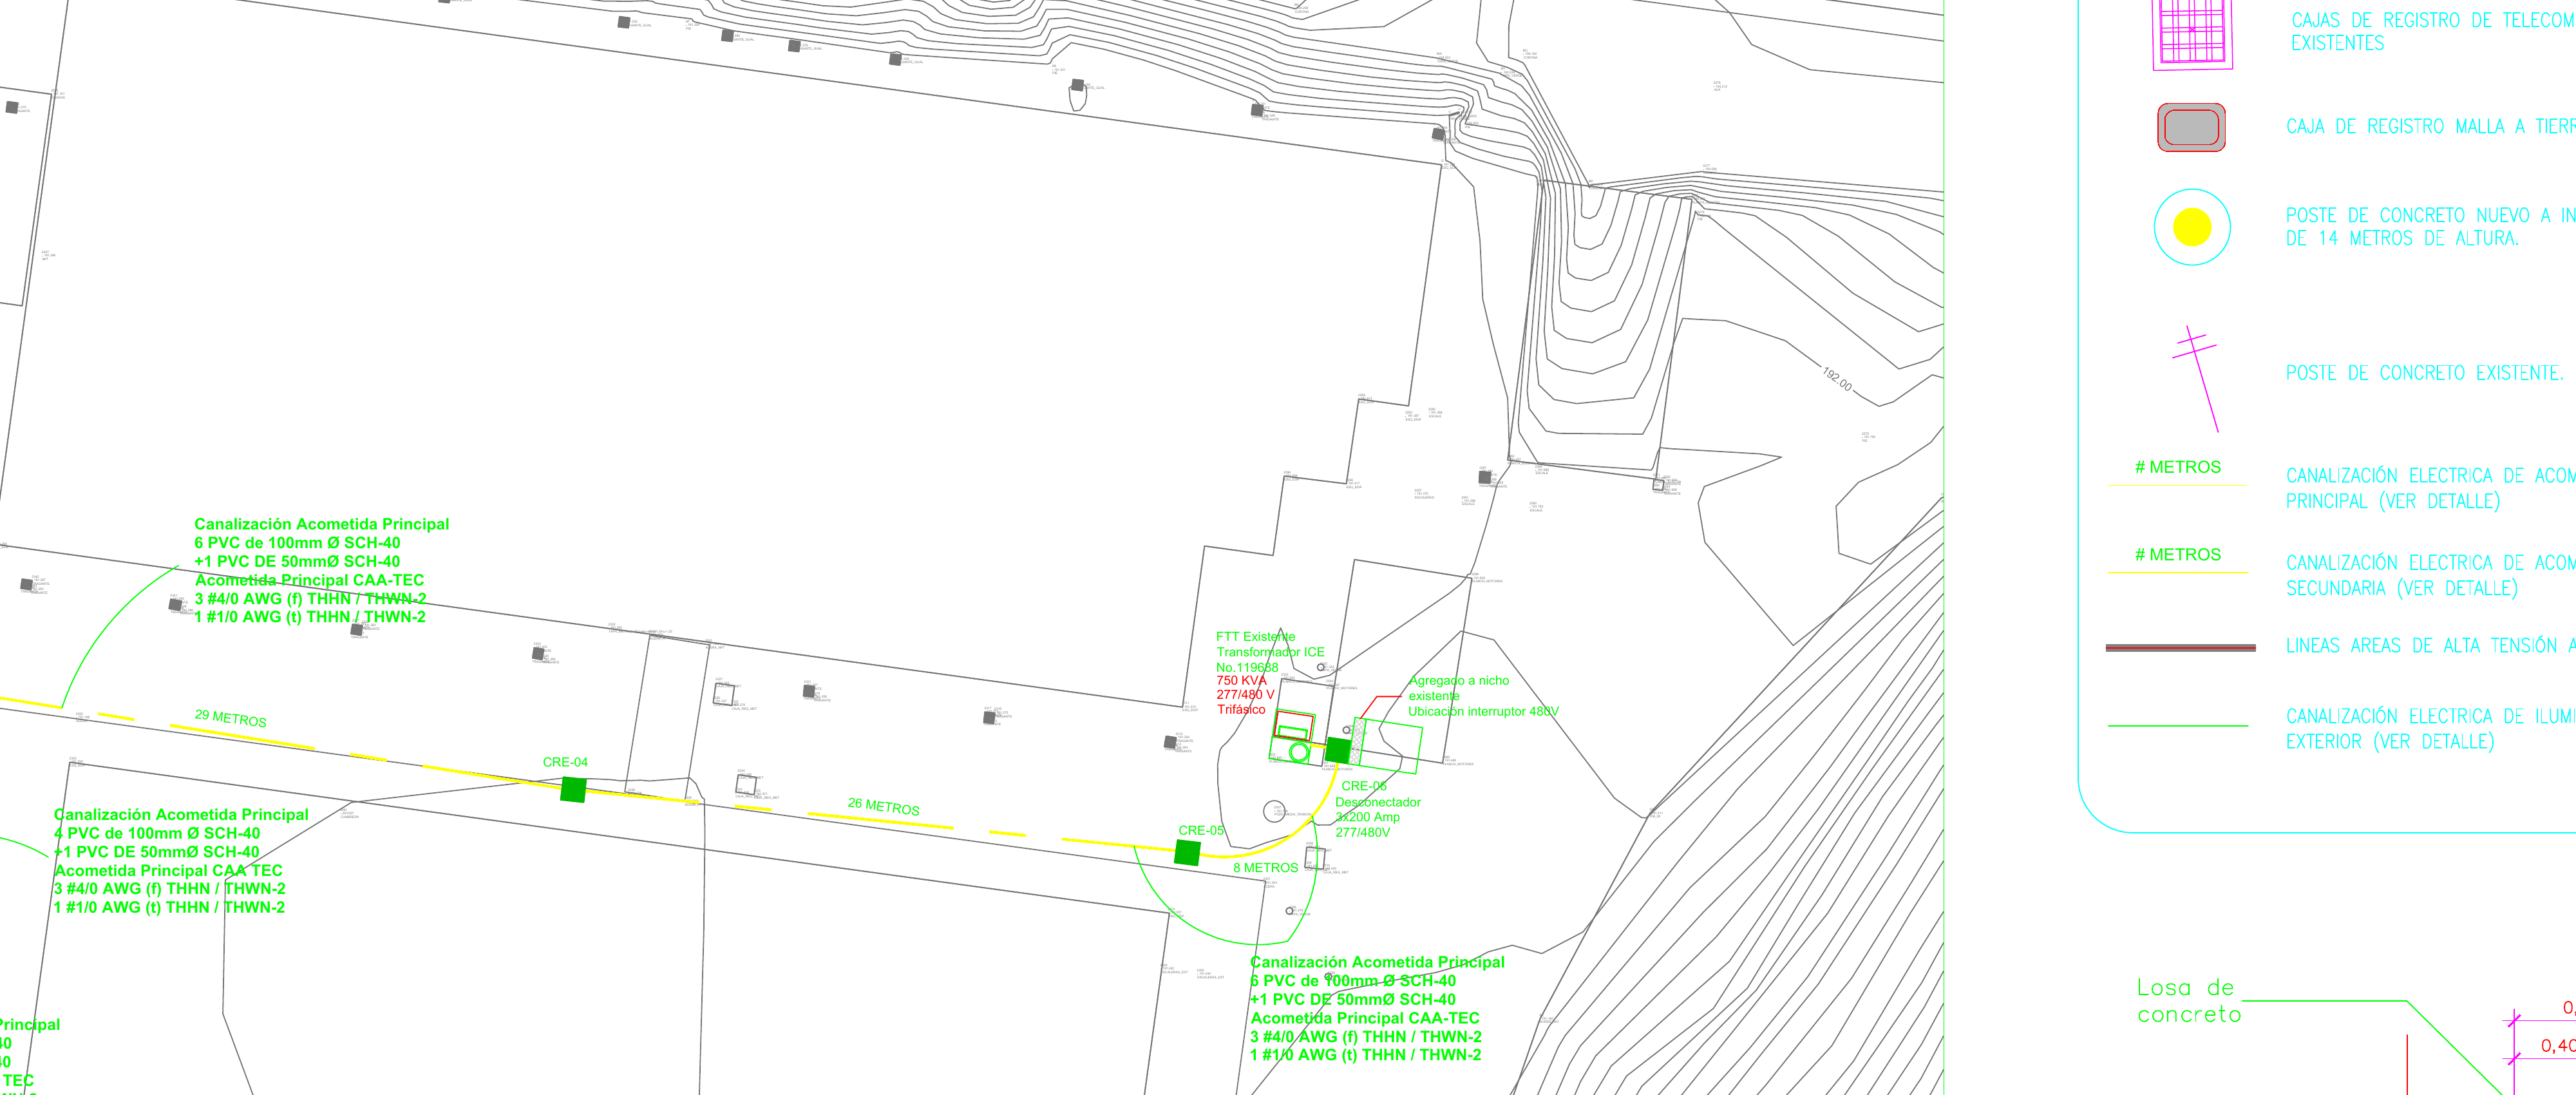
\includegraphics[width=0.92\textwidth]{figuras/acometida.png}
\caption{Lámina E01 (as-built del CAA): transformador del ICE N.\textsuperscript{o} 119688, nicho del interruptor de 480~V y canalización de la acometida existente \cite{p2}.}
\end{figure}
\begin{figure}[H]
\centering
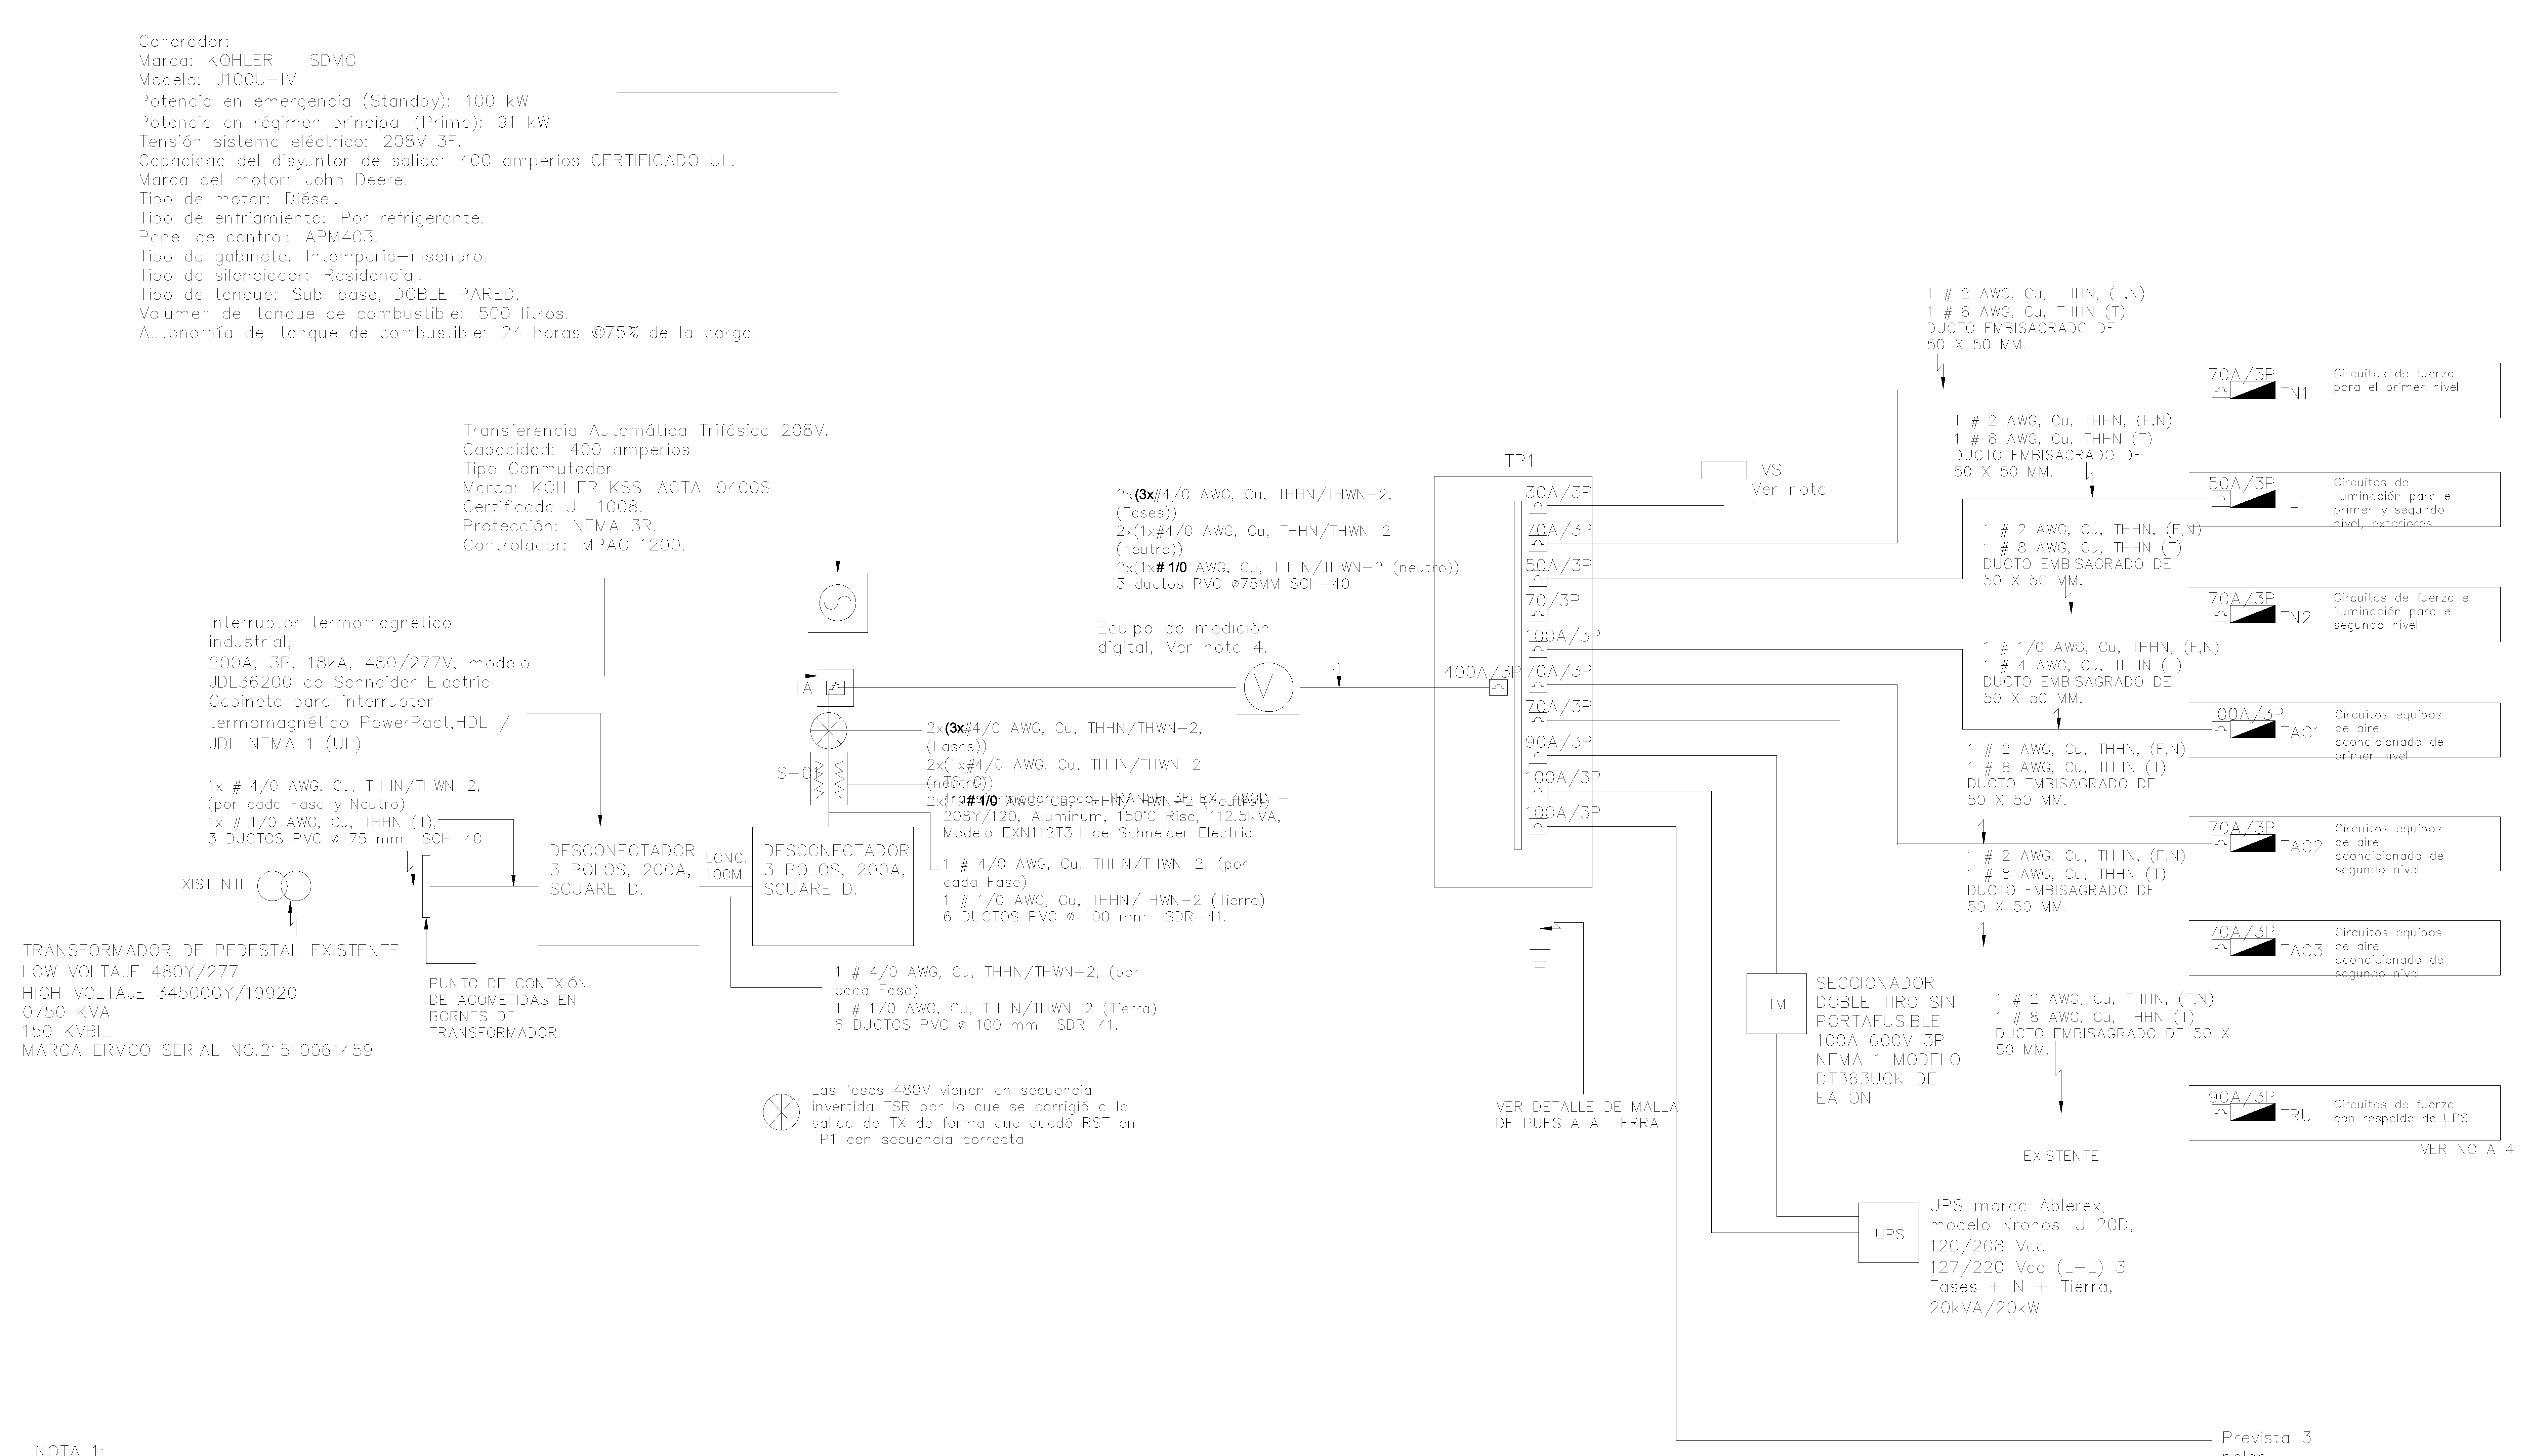
\includegraphics[width=0.92\textwidth]{figuras/unifilar_existente_bn.png}
\caption{Unifilar existente del CAA (E07): la estación no toma carga de TS-01 ni del TP, sino de un servicio nuevo en el nicho del transformador \cite{p2}.}
\end{figure}

\section{Registro de uso de inteligencia artificial}
\label{sec:ia}
% Registro de uso de IA (exigido por el enunciado)
El enunciado permite usar herramientas de inteligencia artificial si la información se verifica con fuentes confiables, y exige incluir íntegramente los prompts. En este proyecto se usó \textbf{Claude} (Anthropic), en la herramienta Claude Code, como asistente para buscar fuentes, organizar la investigación, programar los cálculos y redactar las láminas y el documento. Toda la información técnica y normativa se contrastó con las fuentes citadas: fichas de los fabricantes, La Gaceta, ARESEP, INTECO, el ICE y el NEC. Los datos que no se pudieron verificar se marcaron como supuestos \supuesto{} o se eliminaron del texto; por ejemplo, la potencia V2L del Ioniq~5.

\subsection*{Prompt del grupo a Claude (íntegro)}
\begin{quote}\itshape
hola en la carpeta anterior esta la estructura de los 2 proyectos anteriores, revisalos para que mires como se trabajo y como debes trabjarlo para este tercero, creo que este tercero se parece mas al 1ro, el caso es que necesito que lo hagas, busca en linea un posible lugar que sea viable, si puedes encontrar los planos o descargarlo tu mismo, entonces porfavor empieza
\end{quote}
Ante la pregunta del asistente sobre el sitio, el grupo eligió la opción ``Parqueo UTN/CAA (Recomendado)''.

\subsection*{Consultas de búsqueda generadas por la herramienta}
Para trazabilidad, se listan las consultas que la herramienta hizo en la web. Sus resultados se usaron solo después de leer la fuente primaria citada.
{\small
\begin{enumerate}
\item planos tipo vivienda interés social Costa Rica pdf descargar BANHVI INVU
\item planos arquitectónicos públicos licitación SICOP estacionamiento Costa Rica pdf planta parqueo
\item Ley 9518 incentivos transporte eléctrico reforma Ley 10209 centros de recarga artículo
\item Decreto Ejecutivo 41642-MINAE reglamento construcción y funcionamiento red centros de recarga eléctrica distribuidoras
\item INTE N121 INTE N120 norma infraestructura recarga vehículos eléctricos Costa Rica INTECO
\item ARESEP tarifa centros de recarga rápida vehículos eléctricos 2026 ₡/kWh ICE CNFL
\item ``41642-MINAE'' centros de recarga reglamento 2019 La Gaceta conectores
\item ``INTE N121'' OR ``INTE N 121'' OR ``INTE N120'' vehículos eléctricos estaciones de carga señalización
\item red de carga rápida ICE conectores CCS1 CHAdeMO tipo 2 GB/T cargadores Costa Rica 2026
\item vehículos eléctricos más vendidos Costa Rica 2026 BYD conector CCS2 tipo 2 mercado
\item BYD Dolphin Costa Rica ficha técnica puerto de carga GB/T CCS2 tipo 2 kW
\item cargador rápido DC 60 kW CCS1 GB/T CHAdeMO 480V UL listed datasheet dual connector
\item ABB Terra 54 UL 480V CCS1 CHAdeMO datasheet input current specifications pdf
\item Costa Rica cargadores vehículos eléctricos venta wallbox precio ChargePoint ABB Autel distribuidor 2026
\item ELCO Costa Rica cargador vehículo eléctrico GB/T J1772 modelo kW ficha técnica
\item 7kW GB/T AC wallbox charger datasheet pdf GB/T 20234.2 IEC 61851-1 single phase 32A CE certified
\item Autel MaxiCharger AC Elite Business 40A spec sheet pdf UL 2594 OCPP RFID dual
\item F-150 Lightning Pro Power Onboard 9.6 kW charge another electric vehicle Mobile Power Cord owner manual V2V Ford
\item vehicle-to-vehicle charging adapter Lucid RangeXchange Cybertruck Powershare V2V GM V2V adapter kW official
\item Reglamento Ley 7600 Decreto 26831 estacionamiento personas con discapacidad dimensiones 3,30 m 5 \% artículo
\item Reglamento de Construcciones INVU 2018 dimensiones espacio estacionamiento 2,50 m x 5,00 m pasillo circulación 90 grados
\item Autel MaxiCharger DC Fast 60kW price USD
\item Ford Mobile Power Cord F-150 Lightning price accessory 32A 240V 120V
\item Ley 9518 texto ``centros de recarga'' artículo 30 31 32 33 instituciones públicas estacionamientos preferenciales vehículos eléctricos reglamento 41092
\item 2024 Hyundai Ioniq 5 long range 77.4 kWh onboard charger 10.9 kW 10-80\% 18 minutes V2L 1.9 kW specifications
\item 2024 F-150 Lightning extended range 131 kWh usable 19.2 kW onboard charger 48A 11.3 kW DC fast charge 15-80\% 41 minutes specifications
\item Nissan Leaf S 40 kWh 6.6 kW onboard charger CHAdeMO 50 kW 2023 specifications; Tesla Model Y Long Range onboard charger 11.5 kW 48A 250 kW
\end{enumerate}}

\subsection*{Verificación aplicada}
\begin{itemize}
\item Leyes y decretos: se confirmaron con La Gaceta (Decreto 41428, en \texttt{Datasheets/}) y con dos fuentes independientes para la Ley 10937. Las discrepancias, como el plazo de ARESEP, se declaran en el texto.
\item Equipos: todos los datos eléctricos de los equipos seleccionados salen de sus fichas en PDF, archivadas en \texttt{Datasheets/}.
\item Cálculos: se revisaron a mano para un caso de cada tipo (sección~\ref{sec:calc_carga}) y con las tablas del NEC 2020.
\item Imagen del sitio: se descargó del servicio Esri World Imagery y se georreferenció con la escala del mosaico (0,294~m por píxel) y con las dimensiones conocidas del CAA y de la nave del Proyecto~2.
\end{itemize}

\textbf{Nota para el grupo:} cada integrante que use IA para su parte de la presentación debe agregar aquí sus propios prompts, íntegros, antes de la entrega.


\end{document}
